% Options for packages loaded elsewhere
\PassOptionsToPackage{unicode}{hyperref}
\PassOptionsToPackage{hyphens}{url}
\PassOptionsToPackage{dvipsnames,svgnames,x11names}{xcolor}
%
\documentclass[
  letterpaper,
  DIV=11,
  numbers=noendperiod]{scrartcl}

\usepackage{amsmath,amssymb}
\usepackage{iftex}
\ifPDFTeX
  \usepackage[T1]{fontenc}
  \usepackage[utf8]{inputenc}
  \usepackage{textcomp} % provide euro and other symbols
\else % if luatex or xetex
  \usepackage{unicode-math}
  \defaultfontfeatures{Scale=MatchLowercase}
  \defaultfontfeatures[\rmfamily]{Ligatures=TeX,Scale=1}
\fi
\usepackage{lmodern}
\ifPDFTeX\else  
    % xetex/luatex font selection
\fi
% Use upquote if available, for straight quotes in verbatim environments
\IfFileExists{upquote.sty}{\usepackage{upquote}}{}
\IfFileExists{microtype.sty}{% use microtype if available
  \usepackage[]{microtype}
  \UseMicrotypeSet[protrusion]{basicmath} % disable protrusion for tt fonts
}{}
\makeatletter
\@ifundefined{KOMAClassName}{% if non-KOMA class
  \IfFileExists{parskip.sty}{%
    \usepackage{parskip}
  }{% else
    \setlength{\parindent}{0pt}
    \setlength{\parskip}{6pt plus 2pt minus 1pt}}
}{% if KOMA class
  \KOMAoptions{parskip=half}}
\makeatother
\usepackage{xcolor}
\setlength{\emergencystretch}{3em} % prevent overfull lines
\setcounter{secnumdepth}{-\maxdimen} % remove section numbering
% Make \paragraph and \subparagraph free-standing
\ifx\paragraph\undefined\else
  \let\oldparagraph\paragraph
  \renewcommand{\paragraph}[1]{\oldparagraph{#1}\mbox{}}
\fi
\ifx\subparagraph\undefined\else
  \let\oldsubparagraph\subparagraph
  \renewcommand{\subparagraph}[1]{\oldsubparagraph{#1}\mbox{}}
\fi

\usepackage{color}
\usepackage{fancyvrb}
\newcommand{\VerbBar}{|}
\newcommand{\VERB}{\Verb[commandchars=\\\{\}]}
\DefineVerbatimEnvironment{Highlighting}{Verbatim}{commandchars=\\\{\}}
% Add ',fontsize=\small' for more characters per line
\usepackage{framed}
\definecolor{shadecolor}{RGB}{241,243,245}
\newenvironment{Shaded}{\begin{snugshade}}{\end{snugshade}}
\newcommand{\AlertTok}[1]{\textcolor[rgb]{0.68,0.00,0.00}{#1}}
\newcommand{\AnnotationTok}[1]{\textcolor[rgb]{0.37,0.37,0.37}{#1}}
\newcommand{\AttributeTok}[1]{\textcolor[rgb]{0.40,0.45,0.13}{#1}}
\newcommand{\BaseNTok}[1]{\textcolor[rgb]{0.68,0.00,0.00}{#1}}
\newcommand{\BuiltInTok}[1]{\textcolor[rgb]{0.00,0.23,0.31}{#1}}
\newcommand{\CharTok}[1]{\textcolor[rgb]{0.13,0.47,0.30}{#1}}
\newcommand{\CommentTok}[1]{\textcolor[rgb]{0.37,0.37,0.37}{#1}}
\newcommand{\CommentVarTok}[1]{\textcolor[rgb]{0.37,0.37,0.37}{\textit{#1}}}
\newcommand{\ConstantTok}[1]{\textcolor[rgb]{0.56,0.35,0.01}{#1}}
\newcommand{\ControlFlowTok}[1]{\textcolor[rgb]{0.00,0.23,0.31}{#1}}
\newcommand{\DataTypeTok}[1]{\textcolor[rgb]{0.68,0.00,0.00}{#1}}
\newcommand{\DecValTok}[1]{\textcolor[rgb]{0.68,0.00,0.00}{#1}}
\newcommand{\DocumentationTok}[1]{\textcolor[rgb]{0.37,0.37,0.37}{\textit{#1}}}
\newcommand{\ErrorTok}[1]{\textcolor[rgb]{0.68,0.00,0.00}{#1}}
\newcommand{\ExtensionTok}[1]{\textcolor[rgb]{0.00,0.23,0.31}{#1}}
\newcommand{\FloatTok}[1]{\textcolor[rgb]{0.68,0.00,0.00}{#1}}
\newcommand{\FunctionTok}[1]{\textcolor[rgb]{0.28,0.35,0.67}{#1}}
\newcommand{\ImportTok}[1]{\textcolor[rgb]{0.00,0.46,0.62}{#1}}
\newcommand{\InformationTok}[1]{\textcolor[rgb]{0.37,0.37,0.37}{#1}}
\newcommand{\KeywordTok}[1]{\textcolor[rgb]{0.00,0.23,0.31}{#1}}
\newcommand{\NormalTok}[1]{\textcolor[rgb]{0.00,0.23,0.31}{#1}}
\newcommand{\OperatorTok}[1]{\textcolor[rgb]{0.37,0.37,0.37}{#1}}
\newcommand{\OtherTok}[1]{\textcolor[rgb]{0.00,0.23,0.31}{#1}}
\newcommand{\PreprocessorTok}[1]{\textcolor[rgb]{0.68,0.00,0.00}{#1}}
\newcommand{\RegionMarkerTok}[1]{\textcolor[rgb]{0.00,0.23,0.31}{#1}}
\newcommand{\SpecialCharTok}[1]{\textcolor[rgb]{0.37,0.37,0.37}{#1}}
\newcommand{\SpecialStringTok}[1]{\textcolor[rgb]{0.13,0.47,0.30}{#1}}
\newcommand{\StringTok}[1]{\textcolor[rgb]{0.13,0.47,0.30}{#1}}
\newcommand{\VariableTok}[1]{\textcolor[rgb]{0.07,0.07,0.07}{#1}}
\newcommand{\VerbatimStringTok}[1]{\textcolor[rgb]{0.13,0.47,0.30}{#1}}
\newcommand{\WarningTok}[1]{\textcolor[rgb]{0.37,0.37,0.37}{\textit{#1}}}

\providecommand{\tightlist}{%
  \setlength{\itemsep}{0pt}\setlength{\parskip}{0pt}}\usepackage{longtable,booktabs,array}
\usepackage{calc} % for calculating minipage widths
% Correct order of tables after \paragraph or \subparagraph
\usepackage{etoolbox}
\makeatletter
\patchcmd\longtable{\par}{\if@noskipsec\mbox{}\fi\par}{}{}
\makeatother
% Allow footnotes in longtable head/foot
\IfFileExists{footnotehyper.sty}{\usepackage{footnotehyper}}{\usepackage{footnote}}
\makesavenoteenv{longtable}
\usepackage{graphicx}
\makeatletter
\def\maxwidth{\ifdim\Gin@nat@width>\linewidth\linewidth\else\Gin@nat@width\fi}
\def\maxheight{\ifdim\Gin@nat@height>\textheight\textheight\else\Gin@nat@height\fi}
\makeatother
% Scale images if necessary, so that they will not overflow the page
% margins by default, and it is still possible to overwrite the defaults
% using explicit options in \includegraphics[width, height, ...]{}
\setkeys{Gin}{width=\maxwidth,height=\maxheight,keepaspectratio}
% Set default figure placement to htbp
\makeatletter
\def\fps@figure{htbp}
\makeatother

\usepackage{booktabs}
\usepackage{longtable}
\usepackage{array}
\usepackage{multirow}
\usepackage{wrapfig}
\usepackage{float}
\usepackage{colortbl}
\usepackage{pdflscape}
\usepackage{tabu}
\usepackage{threeparttable}
\usepackage{threeparttablex}
\usepackage[normalem]{ulem}
\usepackage{makecell}
\usepackage{xcolor}
\KOMAoption{captions}{tableheading}
\makeatletter
\makeatother
\makeatletter
\makeatother
\makeatletter
\@ifpackageloaded{caption}{}{\usepackage{caption}}
\AtBeginDocument{%
\ifdefined\contentsname
  \renewcommand*\contentsname{Table of contents}
\else
  \newcommand\contentsname{Table of contents}
\fi
\ifdefined\listfigurename
  \renewcommand*\listfigurename{List of Figures}
\else
  \newcommand\listfigurename{List of Figures}
\fi
\ifdefined\listtablename
  \renewcommand*\listtablename{List of Tables}
\else
  \newcommand\listtablename{List of Tables}
\fi
\ifdefined\figurename
  \renewcommand*\figurename{Figure}
\else
  \newcommand\figurename{Figure}
\fi
\ifdefined\tablename
  \renewcommand*\tablename{Table}
\else
  \newcommand\tablename{Table}
\fi
}
\@ifpackageloaded{float}{}{\usepackage{float}}
\floatstyle{ruled}
\@ifundefined{c@chapter}{\newfloat{codelisting}{h}{lop}}{\newfloat{codelisting}{h}{lop}[chapter]}
\floatname{codelisting}{Listing}
\newcommand*\listoflistings{\listof{codelisting}{List of Listings}}
\makeatother
\makeatletter
\@ifpackageloaded{caption}{}{\usepackage{caption}}
\@ifpackageloaded{subcaption}{}{\usepackage{subcaption}}
\makeatother
\makeatletter
\@ifpackageloaded{tcolorbox}{}{\usepackage[skins,breakable]{tcolorbox}}
\makeatother
\makeatletter
\@ifundefined{shadecolor}{\definecolor{shadecolor}{rgb}{.97, .97, .97}}
\makeatother
\makeatletter
\makeatother
\makeatletter
\makeatother
\ifLuaTeX
  \usepackage{selnolig}  % disable illegal ligatures
\fi
\IfFileExists{bookmark.sty}{\usepackage{bookmark}}{\usepackage{hyperref}}
\IfFileExists{xurl.sty}{\usepackage{xurl}}{} % add URL line breaks if available
\urlstyle{same} % disable monospaced font for URLs
\hypersetup{
  pdftitle={Mapas e análise exploratória dos dados},
  pdfauthor={Victor Batista},
  colorlinks=true,
  linkcolor={blue},
  filecolor={Maroon},
  citecolor={Blue},
  urlcolor={Blue},
  pdfcreator={LaTeX via pandoc}}

\title{Mapas e análise exploratória dos dados}
\author{Victor Batista}
\date{}

\begin{document}
\maketitle
\ifdefined\Shaded\renewenvironment{Shaded}{\begin{tcolorbox}[interior hidden, sharp corners, enhanced, borderline west={3pt}{0pt}{shadecolor}, breakable, boxrule=0pt, frame hidden]}{\end{tcolorbox}}\fi

\hypertarget{introduuxe7uxe3o}{%
\section{Introdução}\label{introduuxe7uxe3o}}

Configura pacotes, diretórios e insere os dados

\hypertarget{mapas}{%
\section{Mapas}\label{mapas}}

\hypertarget{luxea-os-shapefiles}{%
\subsection{Lê os shapefiles}\label{luxea-os-shapefiles}}

\begin{Shaded}
\begin{Highlighting}[]
\NormalTok{fronteira }\OtherTok{\textless{}{-}} \FunctionTok{st\_read}\NormalTok{(}\FunctionTok{file.path}\NormalTok{(dropbox,}\StringTok{"Fronteira/Faixa\_de\_Fronteira\_por\_UF\_2022.shp"}\NormalTok{)) }\SpecialCharTok{\%\textgreater{}\%}
  \FunctionTok{st\_transform}\NormalTok{(}\StringTok{"WGS84"}\NormalTok{)}
\end{Highlighting}
\end{Shaded}

\begin{verbatim}
Reading layer `Faixa_de_Fronteira_por_UF_2022' from data source 
  `C:\Users\victo\Dropbox\DISSERTACAO\Fronteira\Faixa_de_Fronteira_por_UF_2022.shp' 
  using driver `ESRI Shapefile'
Simple feature collection with 11 features and 7 fields
Geometry type: MULTIPOLYGON
Dimension:     XY
Bounding box:  xmin: -73.99045 ymin: -33.75118 xmax: -50.91768 ymax: 5.271841
Geodetic CRS:  SIRGAS 2000
\end{verbatim}

\begin{Shaded}
\begin{Highlighting}[]
\FunctionTok{tm\_shape}\NormalTok{(fronteira, }\AttributeTok{unit =} \StringTok{"km"}\NormalTok{)}\SpecialCharTok{+}
  \FunctionTok{tm\_fill}\NormalTok{(}\AttributeTok{alpha =} \FloatTok{0.7}\NormalTok{) }\SpecialCharTok{+} 
  \FunctionTok{tm\_borders}\NormalTok{(}\AttributeTok{col =} \StringTok{"black"}\NormalTok{)}
\end{Highlighting}
\end{Shaded}

\begin{figure}[H]

{\centering 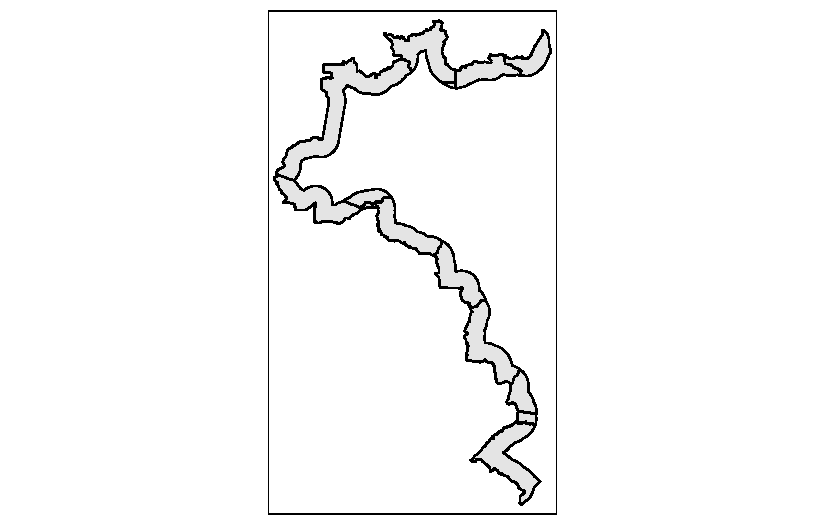
\includegraphics{maps_files/figure-pdf/shapefilefronteira-1.pdf}

}

\end{figure}

\hypertarget{uniformiza-a-faixa-de-fronteira-como-uma-uxfanica-regiuxe3o}{%
\subsection{Uniformiza a faixa de fronteira como uma única
região}\label{uniformiza-a-faixa-de-fronteira-como-uma-uxfanica-regiuxe3o}}

\begin{Shaded}
\begin{Highlighting}[]
\NormalTok{linha\_fronteira }\OtherTok{\textless{}{-}}\NormalTok{ fronteira }\SpecialCharTok{\%\textgreater{}\%}
  \FunctionTok{mutate}\NormalTok{(}\AttributeTok{pais =} \StringTok{"BR"}\NormalTok{) }\SpecialCharTok{\%\textgreater{}\%} 
  \FunctionTok{group\_by}\NormalTok{(pais) }\SpecialCharTok{\%\textgreater{}\%} 
  \FunctionTok{summarise}\NormalTok{()}

\FunctionTok{tm\_shape}\NormalTok{(linha\_fronteira, }\AttributeTok{unit =} \StringTok{"km"}\NormalTok{)}\SpecialCharTok{+}
  \FunctionTok{tm\_fill}\NormalTok{(}\AttributeTok{alpha =} \FloatTok{0.7}\NormalTok{) }\SpecialCharTok{+} 
  \FunctionTok{tm\_borders}\NormalTok{(}\AttributeTok{col =} \StringTok{"black"}\NormalTok{)}
\end{Highlighting}
\end{Shaded}

\begin{figure}[H]

{\centering \includegraphics{maps_files/figure-pdf/sflinha-1.pdf}

}

\end{figure}

\hypertarget{carrega-sf-dos-municuxedpios-brasileiros}{%
\subsection{Carrega sf dos municípios
brasileiros}\label{carrega-sf-dos-municuxedpios-brasileiros}}

\begin{Shaded}
\begin{Highlighting}[]
\NormalTok{municipios }\OtherTok{\textless{}{-}} \FunctionTok{read\_municipality}\NormalTok{(}\AttributeTok{year=}\DecValTok{2020}\NormalTok{, }\AttributeTok{showProgress =}\NormalTok{ T) }\SpecialCharTok{\%\textgreater{}\%}
  \FunctionTok{st\_transform}\NormalTok{(}\StringTok{"WGS84"}\NormalTok{)}
\end{Highlighting}
\end{Shaded}

\begin{verbatim}
Using year/date 2020
\end{verbatim}

\begin{verbatim}

  |                                                                            
  |                                                                      |   0%
  |                                                                            
  |===                                                                   |   4%
  |                                                                            
  |=====                                                                 |   7%
  |                                                                            
  |========                                                              |  11%
  |                                                                            
  |==========                                                            |  15%
  |                                                                            
  |=============                                                         |  19%
  |                                                                            
  |================                                                      |  22%
  |                                                                            
  |==================                                                    |  26%
  |                                                                            
  |=====================                                                 |  30%
  |                                                                            
  |=======================                                               |  33%
  |                                                                            
  |==========================                                            |  37%
  |                                                                            
  |=============================                                         |  41%
  |                                                                            
  |===============================                                       |  44%
  |                                                                            
  |==================================                                    |  48%
  |                                                                            
  |====================================                                  |  52%
  |                                                                            
  |=======================================                               |  56%
  |                                                                            
  |=========================================                             |  59%
  |                                                                            
  |============================================                          |  63%
  |                                                                            
  |===============================================                       |  67%
  |                                                                            
  |=================================================                     |  70%
  |                                                                            
  |====================================================                  |  74%
  |                                                                            
  |======================================================                |  78%
  |                                                                            
  |=========================================================             |  81%
  |                                                                            
  |============================================================          |  85%
  |                                                                            
  |==============================================================        |  89%
  |                                                                            
  |=================================================================     |  93%
  |                                                                            
  |===================================================================   |  96%
  |                                                                            
  |======================================================================| 100%
\end{verbatim}

\begin{Shaded}
\begin{Highlighting}[]
\FunctionTok{tm\_shape}\NormalTok{(municipios, }\AttributeTok{unit =} \StringTok{"km"}\NormalTok{)}\SpecialCharTok{+}
  \FunctionTok{tm\_fill}\NormalTok{(}\AttributeTok{alpha =} \FloatTok{0.7}\NormalTok{) }\SpecialCharTok{+} 
  \FunctionTok{tm\_borders}\NormalTok{(}\AttributeTok{col =} \StringTok{"black"}\NormalTok{)}
\end{Highlighting}
\end{Shaded}

\begin{figure}[H]

{\centering \includegraphics{maps_files/figure-pdf/sfmunicipios-1.pdf}

}

\end{figure}

\hypertarget{carrega-o-sf-dos-pauxedses-da-amuxe9rica-do-sul}{%
\subsection{Carrega o sf dos países da América do
Sul}\label{carrega-o-sf-dos-pauxedses-da-amuxe9rica-do-sul}}

\begin{Shaded}
\begin{Highlighting}[]
\NormalTok{america }\OtherTok{\textless{}{-}} \FunctionTok{st\_read}\NormalTok{(}\FunctionTok{file.path}\NormalTok{(dropbox,}\StringTok{"America/South\_America.shp"}\NormalTok{)) }\SpecialCharTok{\%\textgreater{}\%} 
  \FunctionTok{st\_transform}\NormalTok{(}\StringTok{"WGS84"}\NormalTok{)}
\end{Highlighting}
\end{Shaded}

\begin{verbatim}
Reading layer `South_America' from data source 
  `C:\Users\victo\Dropbox\DISSERTACAO\America\South_America.shp' 
  using driver `ESRI Shapefile'
Simple feature collection with 15 features and 1 field
Geometry type: MULTIPOLYGON
Dimension:     XY
Bounding box:  xmin: -109.4461 ymin: -58.49861 xmax: -26.24139 ymax: 12.59028
Geodetic CRS:  WGS 84
\end{verbatim}

\begin{Shaded}
\begin{Highlighting}[]
\FunctionTok{tm\_shape}\NormalTok{(america, }\AttributeTok{unit =} \StringTok{"km"}\NormalTok{)}\SpecialCharTok{+}
  \FunctionTok{tm\_fill}\NormalTok{(}\AttributeTok{alpha =} \FloatTok{0.7}\NormalTok{) }\SpecialCharTok{+} 
  \FunctionTok{tm\_borders}\NormalTok{(}\AttributeTok{col =} \StringTok{"black"}\NormalTok{)}
\end{Highlighting}
\end{Shaded}

\begin{figure}[H]

{\centering \includegraphics{maps_files/figure-pdf/sfamerica-1.pdf}

}

\end{figure}

\hypertarget{carrega-o-sf-dos-municuxedpios-da-faixa-de-fronteira}{%
\subsection{Carrega o sf dos municípios da faixa de
fronteira}\label{carrega-o-sf-dos-municuxedpios-da-faixa-de-fronteira}}

\begin{Shaded}
\begin{Highlighting}[]
\NormalTok{municipios\_fronteira }\OtherTok{\textless{}{-}} \FunctionTok{st\_read}\NormalTok{(}\FunctionTok{file.path}\NormalTok{(dropbox,}\StringTok{"Municipios\_Fronteira/Municipios\_Faixa\_Fronteira\_2022.shp"}\NormalTok{)) }\SpecialCharTok{\%\textgreater{}\%}
  \FunctionTok{st\_transform}\NormalTok{(}\StringTok{"WGS84"}\NormalTok{)}
\end{Highlighting}
\end{Shaded}

\begin{verbatim}
Reading layer `Municipios_Faixa_Fronteira_2022' from data source 
  `C:\Users\victo\Dropbox\DISSERTACAO\Municipios_Fronteira\Municipios_Faixa_Fronteira_2022.shp' 
  using driver `ESRI Shapefile'
Simple feature collection with 590 features and 10 fields
Geometry type: MULTIPOLYGON
Dimension:     XY
Bounding box:  xmin: -73.99045 ymin: -33.75118 xmax: -49.87568 ymax: 5.271841
Geodetic CRS:  SIRGAS 2000
\end{verbatim}

\begin{Shaded}
\begin{Highlighting}[]
\FunctionTok{tm\_shape}\NormalTok{(municipios\_fronteira, }\AttributeTok{unit =} \StringTok{"km"}\NormalTok{)}\SpecialCharTok{+}
  \FunctionTok{tm\_fill}\NormalTok{(}\AttributeTok{alpha =} \FloatTok{0.7}\NormalTok{) }\SpecialCharTok{+} 
  \FunctionTok{tm\_borders}\NormalTok{(}\AttributeTok{col =} \StringTok{"black"}\NormalTok{)}
\end{Highlighting}
\end{Shaded}

\begin{figure}[H]

{\centering \includegraphics{maps_files/figure-pdf/sfmunicipiosff-1.pdf}

}

\end{figure}

\hypertarget{novos-municuxedpios-propostos}{%
\subsection{Novos municípios
propostos}\label{novos-municuxedpios-propostos}}

\begin{Shaded}
\begin{Highlighting}[]
\CommentTok{\# Estabelece a nova proposta de faixa de fronteira}
\NormalTok{linha\_fronteira\_300km }\OtherTok{\textless{}{-}} \FunctionTok{st\_buffer}\NormalTok{(linha\_fronteira, }\AttributeTok{dist =} \DecValTok{150000}\NormalTok{)}

\CommentTok{\# Verifica municípios que passam a pertencer à região}
\CommentTok{\# Adiciona variável de intercessão}
\NormalTok{municipios}\SpecialCharTok{$}\NormalTok{inter }\OtherTok{\textless{}{-}} \FunctionTok{st\_intersects}\NormalTok{(municipios, linha\_fronteira\_300km, }\AttributeTok{sparse =}\NormalTok{ F)}
\FunctionTok{table}\NormalTok{(municipios}\SpecialCharTok{$}\NormalTok{inter)}
\end{Highlighting}
\end{Shaded}

\begin{verbatim}

FALSE  TRUE 
 4438  1132 
\end{verbatim}

\hypertarget{faixa-de-fronteira-original}{%
\subsection{Faixa de fronteira
original}\label{faixa-de-fronteira-original}}

\begin{Shaded}
\begin{Highlighting}[]
\CommentTok{\# Adiciona variável de pertencimento à fronteira original}
\NormalTok{municipios }\OtherTok{\textless{}{-}}\NormalTok{ municipios }\SpecialCharTok{\%\textgreater{}\%}
  \FunctionTok{mutate}\NormalTok{(}\AttributeTok{fronteira =} \FunctionTok{ifelse}\NormalTok{(code\_muni }\SpecialCharTok{\%in\%}\NormalTok{ municipios\_fronteira}\SpecialCharTok{$}\NormalTok{CD\_MUN, }\DecValTok{1}\NormalTok{, }\DecValTok{0}\NormalTok{))}
\FunctionTok{table}\NormalTok{(municipios}\SpecialCharTok{$}\NormalTok{fronteira)}
\end{Highlighting}
\end{Shaded}

\begin{verbatim}

   0    1 
4982  588 
\end{verbatim}

\hypertarget{criauxe7uxe3o-de-tratamento-e-controle}{%
\section{Criação de tratamento e
controle}\label{criauxe7uxe3o-de-tratamento-e-controle}}

\begin{Shaded}
\begin{Highlighting}[]
\NormalTok{df }\OtherTok{\textless{}{-}}\NormalTok{ municipios }\SpecialCharTok{|\textgreater{}}
  \CommentTok{\#filtra os municípios na nova faixa}
  \FunctionTok{filter}\NormalTok{(inter }\SpecialCharTok{==}\NormalTok{ T) }\SpecialCharTok{|\textgreater{}} 
  \CommentTok{\# cria o grupo de tratamento e controle}
  \FunctionTok{mutate}\NormalTok{(}\AttributeTok{treated =} \FunctionTok{ifelse}\NormalTok{(code\_muni }\SpecialCharTok{\%in\%}\NormalTok{ municipios\_fronteira}\SpecialCharTok{$}\NormalTok{CD\_MUN, }\DecValTok{1}\NormalTok{, }\DecValTok{0}\NormalTok{),}
         \AttributeTok{groups =} \FunctionTok{ifelse}\NormalTok{(treated }\SpecialCharTok{==} \DecValTok{1}\NormalTok{, }\StringTok{"treatment"}\NormalTok{, }\StringTok{"control"}\NormalTok{),}
         \CommentTok{\# cria os arcos}
         \AttributeTok{arcos =} \FunctionTok{case\_when}\NormalTok{(abbrev\_state }\SpecialCharTok{\%in\%} \FunctionTok{c}\NormalTok{(}\StringTok{"AP"}\NormalTok{, }\StringTok{"PA"}\NormalTok{, }\StringTok{"AM"}\NormalTok{, }\StringTok{"AC"}\NormalTok{, }\StringTok{"RR"}\NormalTok{) }\SpecialCharTok{\textasciitilde{}} \StringTok{"Arco Norte"}\NormalTok{,}
\NormalTok{                           abbrev\_state }\SpecialCharTok{\%in\%} \FunctionTok{c}\NormalTok{(}\StringTok{"RO"}\NormalTok{, }\StringTok{"MS"}\NormalTok{, }\StringTok{"MT"}\NormalTok{) }\SpecialCharTok{\textasciitilde{}} \StringTok{"Arco Central"}\NormalTok{,}
\NormalTok{                           abbrev\_state }\SpecialCharTok{\%in\%} \FunctionTok{c}\NormalTok{(}\StringTok{"PR"}\NormalTok{, }\StringTok{"SC"}\NormalTok{, }\StringTok{"RS"}\NormalTok{) }\SpecialCharTok{\textasciitilde{}} \StringTok{"Arco Sul"}\NormalTok{)) }\SpecialCharTok{|\textgreater{}} 
  \CommentTok{\# exclui a variável classificatória. as recém criadas a substituem}
\NormalTok{  dplyr}\SpecialCharTok{::}\FunctionTok{select}\NormalTok{(}\SpecialCharTok{{-}}\NormalTok{inter)}
\end{Highlighting}
\end{Shaded}

\begin{verbatim}
Warning: Using one column matrices in `filter()` was deprecated in dplyr 1.1.0.
i Please use one dimensional logical vectors instead.
\end{verbatim}

\begin{Shaded}
\begin{Highlighting}[]
\FunctionTok{glimpse}\NormalTok{(df)}
\end{Highlighting}
\end{Shaded}

\begin{verbatim}
Rows: 1,132
Columns: 12
$ code_muni    <dbl> 1100015, 1100023, 1100031, 1100049, 1100056, 1100064, 110~
$ name_muni    <chr> "Alta Floresta D'oeste", "Ariquemes", "Cabixi", "Cacoal",~
$ code_state   <dbl> 11, 11, 11, 11, 11, 11, 11, 11, 11, 11, 11, 11, 11, 11, 1~
$ abbrev_state <chr> "RO", "RO", "RO", "RO", "RO", "RO", "RO", "RO", "RO", "RO~
$ name_state   <chr> "Rondônia", "Rondônia", "Rondônia", "Rondônia", "Rondônia~
$ code_region  <dbl> 1, 1, 1, 1, 1, 1, 1, 1, 1, 1, 1, 1, 1, 1, 1, 1, 1, 1, 1, ~
$ name_region  <chr> "Norte", "Norte", "Norte", "Norte", "Norte", "Norte", "No~
$ fronteira    <dbl> 1, 0, 1, 0, 1, 1, 1, 1, 0, 1, 0, 0, 0, 1, 0, 1, 1, 0, 0, ~
$ treated      <dbl> 1, 0, 1, 0, 1, 1, 1, 1, 0, 1, 0, 0, 0, 1, 0, 1, 1, 0, 0, ~
$ groups       <chr> "treatment", "control", "treatment", "control", "treatmen~
$ arcos        <chr> "Arco Central", "Arco Central", "Arco Central", "Arco Cen~
$ geom         <MULTIPOLYGON [°]> MULTIPOLYGON (((-62.19465 -..., MULTIPOLYGON~
\end{verbatim}

\begin{Shaded}
\begin{Highlighting}[]
\CommentTok{\# prepara a tabela da fronteira para mergir com a df principal (municipios)}
\NormalTok{t }\OtherTok{\textless{}{-}}\NormalTok{ municipios\_fronteira }\SpecialCharTok{|\textgreater{}} 
  \CommentTok{\# remove colunas indesejadas}
  \FunctionTok{select}\NormalTok{(}\SpecialCharTok{{-}}\FunctionTok{c}\NormalTok{(}\StringTok{"NM\_REGIAO"}\NormalTok{, }\StringTok{"CD\_UF"}\NormalTok{, }\StringTok{"NM\_UF"}\NormalTok{, }\StringTok{"SIGLA\_UF"}\NormalTok{, }\StringTok{"NM\_MUN"}\NormalTok{, }\StringTok{"geometry"}\NormalTok{)) }\SpecialCharTok{|\textgreater{}} 
  \CommentTok{\# padroniza o nome code\_muni}
  \FunctionTok{rename}\NormalTok{(}\StringTok{"code\_muni"} \OtherTok{=} \StringTok{"CD\_MUN"}\NormalTok{) }\SpecialCharTok{|\textgreater{}} 
  \CommentTok{\# altera o tipo das colunas para numeric e logic}
  \FunctionTok{mutate}\NormalTok{(}\AttributeTok{code\_muni =} \FunctionTok{as.numeric}\NormalTok{(code\_muni),}
         \AttributeTok{CID\_GEMEA =} \FunctionTok{ifelse}\NormalTok{(}\FunctionTok{is.na}\NormalTok{(CID\_GEMEA) }\SpecialCharTok{==}\NormalTok{ F, }\DecValTok{1}\NormalTok{, }\DecValTok{0}\NormalTok{))}

\CommentTok{\# remove o componente gráfico}
\FunctionTok{st\_geometry}\NormalTok{(t) }\OtherTok{\textless{}{-}} \ConstantTok{NULL}

\CommentTok{\# realiza o join}
\NormalTok{df }\OtherTok{\textless{}{-}}\NormalTok{ dplyr}\SpecialCharTok{::}\FunctionTok{left\_join}\NormalTok{(df, t, }\AttributeTok{by =} \StringTok{"code\_muni"}\NormalTok{)}
\FunctionTok{rm}\NormalTok{(t)}

\FunctionTok{glimpse}\NormalTok{(df)}
\end{Highlighting}
\end{Shaded}

\begin{verbatim}
Rows: 1,132
Columns: 16
$ code_muni    <dbl> 1100015, 1100023, 1100031, 1100049, 1100056, 1100064, 110~
$ name_muni    <chr> "Alta Floresta D'oeste", "Ariquemes", "Cabixi", "Cacoal",~
$ code_state   <dbl> 11, 11, 11, 11, 11, 11, 11, 11, 11, 11, 11, 11, 11, 11, 1~
$ abbrev_state <chr> "RO", "RO", "RO", "RO", "RO", "RO", "RO", "RO", "RO", "RO~
$ name_state   <chr> "Rondônia", "Rondônia", "Rondônia", "Rondônia", "Rondônia~
$ code_region  <dbl> 1, 1, 1, 1, 1, 1, 1, 1, 1, 1, 1, 1, 1, 1, 1, 1, 1, 1, 1, ~
$ name_region  <chr> "Norte", "Norte", "Norte", "Norte", "Norte", "Norte", "No~
$ fronteira    <dbl> 1, 0, 1, 0, 1, 1, 1, 1, 0, 1, 0, 0, 0, 1, 0, 1, 1, 0, 0, ~
$ treated      <dbl> 1, 0, 1, 0, 1, 1, 1, 1, 0, 1, 0, 0, 0, 1, 0, 1, 1, 0, 0, ~
$ groups       <chr> "treatment", "control", "treatment", "control", "treatmen~
$ arcos        <chr> "Arco Central", "Arco Central", "Arco Central", "Arco Cen~
$ AREA_TOT     <dbl> 7067.127, NA, 1314.352, NA, 2783.300, 1451.060, 3060.321,~
$ AREA_INT     <dbl> 7067.127, NA, 1314.352, NA, 2783.300, 1451.060, 3060.321,~
$ PORC_INT     <dbl> 100.000000, NA, 100.000000, NA, 100.000000, 100.000000, 1~
$ CID_GEMEA    <dbl> 0, NA, 0, NA, 0, 0, 0, 0, NA, 1, NA, NA, NA, 0, NA, 0, 0,~
$ geom         <MULTIPOLYGON [°]> MULTIPOLYGON (((-62.19465 -..., MULTIPOLYGON~
\end{verbatim}

\begin{Shaded}
\begin{Highlighting}[]
\CommentTok{\# prepara a tabela da sede dos mun da faixa da fronteira para mergir com a df principal (municipios)}
\NormalTok{sede\_municipios }\OtherTok{\textless{}{-}} \FunctionTok{st\_read}\NormalTok{(}\FunctionTok{file.path}\NormalTok{(dropbox,}\StringTok{"Sedes\_Municipios\_Faixa\_de\_Fronteira\_Cidades\_Gemeas\_2022\_shp/Sedes\_Municipios\_Faixa\_de\_Fronteira\_Cidades\_Gemeas\_2022.shp"}\NormalTok{)) }\SpecialCharTok{\%\textgreater{}\%}
  \FunctionTok{st\_transform}\NormalTok{(}\StringTok{"WGS84"}\NormalTok{)}
\end{Highlighting}
\end{Shaded}

\begin{verbatim}
Reading layer `Sedes_Municipios_Faixa_de_Fronteira_Cidades_Gemeas_2022' from data source `C:\Users\victo\Dropbox\DISSERTACAO\Sedes_Municipios_Faixa_de_Fronteira_Cidades_Gemeas_2022_shp\Sedes_Municipios_Faixa_de_Fronteira_Cidades_Gemeas_2022.shp' 
  using driver `ESRI Shapefile'
Simple feature collection with 588 features and 10 fields
Geometry type: POINT
Dimension:     XY
Bounding box:  xmin: -72.906 ymin: -33.689 xmax: -50.783 ymax: 4.595
Geodetic CRS:  WGS 84
\end{verbatim}

\begin{Shaded}
\begin{Highlighting}[]
\NormalTok{t }\OtherTok{\textless{}{-}}\NormalTok{ sede\_municipios }\SpecialCharTok{\%\textgreater{}\%}
  \CommentTok{\# seleciona colunas desejadas}
  \FunctionTok{select}\NormalTok{(}\FunctionTok{c}\NormalTok{(}\StringTok{"CD\_MUN"}\NormalTok{, }\StringTok{"FAIXA\_SEDE"}\NormalTok{)) }\SpecialCharTok{\%\textgreater{}\%}
  \CommentTok{\# harmoniza os nomes de variáveis}
  \FunctionTok{rename}\NormalTok{(}\StringTok{"code\_muni"} \OtherTok{=} \StringTok{"CD\_MUN"}\NormalTok{) }\SpecialCharTok{\%\textgreater{}\%}
  \CommentTok{\# modifica a classe da variável}
  \FunctionTok{mutate}\NormalTok{(}\AttributeTok{code\_muni =} \FunctionTok{as.numeric}\NormalTok{(code\_muni),}
         \AttributeTok{FAIXA\_SEDE =} \FunctionTok{ifelse}\NormalTok{(FAIXA\_SEDE }\SpecialCharTok{==} \StringTok{"sim"}\NormalTok{, }\DecValTok{1}\NormalTok{, }\DecValTok{0}\NormalTok{))}

\CommentTok{\# remove a geometria da tabela para realizar o join}
\FunctionTok{st\_geometry}\NormalTok{(t) }\OtherTok{\textless{}{-}} \ConstantTok{NULL}

\CommentTok{\# realiza o join}
\NormalTok{df }\OtherTok{\textless{}{-}}\NormalTok{ dplyr}\SpecialCharTok{::}\FunctionTok{left\_join}\NormalTok{(df, t, }\AttributeTok{by =} \StringTok{"code\_muni"}\NormalTok{)}
\FunctionTok{rm}\NormalTok{(t)}

\FunctionTok{glimpse}\NormalTok{(df)}
\end{Highlighting}
\end{Shaded}

\begin{verbatim}
Rows: 1,132
Columns: 17
$ code_muni    <dbl> 1100015, 1100023, 1100031, 1100049, 1100056, 1100064, 110~
$ name_muni    <chr> "Alta Floresta D'oeste", "Ariquemes", "Cabixi", "Cacoal",~
$ code_state   <dbl> 11, 11, 11, 11, 11, 11, 11, 11, 11, 11, 11, 11, 11, 11, 1~
$ abbrev_state <chr> "RO", "RO", "RO", "RO", "RO", "RO", "RO", "RO", "RO", "RO~
$ name_state   <chr> "Rondônia", "Rondônia", "Rondônia", "Rondônia", "Rondônia~
$ code_region  <dbl> 1, 1, 1, 1, 1, 1, 1, 1, 1, 1, 1, 1, 1, 1, 1, 1, 1, 1, 1, ~
$ name_region  <chr> "Norte", "Norte", "Norte", "Norte", "Norte", "Norte", "No~
$ fronteira    <dbl> 1, 0, 1, 0, 1, 1, 1, 1, 0, 1, 0, 0, 0, 1, 0, 1, 1, 0, 0, ~
$ treated      <dbl> 1, 0, 1, 0, 1, 1, 1, 1, 0, 1, 0, 0, 0, 1, 0, 1, 1, 0, 0, ~
$ groups       <chr> "treatment", "control", "treatment", "control", "treatmen~
$ arcos        <chr> "Arco Central", "Arco Central", "Arco Central", "Arco Cen~
$ AREA_TOT     <dbl> 7067.127, NA, 1314.352, NA, 2783.300, 1451.060, 3060.321,~
$ AREA_INT     <dbl> 7067.127, NA, 1314.352, NA, 2783.300, 1451.060, 3060.321,~
$ PORC_INT     <dbl> 100.000000, NA, 100.000000, NA, 100.000000, 100.000000, 1~
$ CID_GEMEA    <dbl> 0, NA, 0, NA, 0, 0, 0, 0, NA, 1, NA, NA, NA, 0, NA, 0, 0,~
$ FAIXA_SEDE   <dbl> 1, NA, 1, NA, 1, 1, 1, 1, NA, 1, NA, NA, NA, 1, NA, 0, 0,~
$ geom         <MULTIPOLYGON [°]> MULTIPOLYGON (((-62.19465 -..., MULTIPOLYGON~
\end{verbatim}

\begin{Shaded}
\begin{Highlighting}[]
\CommentTok{\# prepara para juntar demais países da américa do sul na base de municípios}
\CommentTok{\# Remove regiões sem fronteira com o br}
\NormalTok{america2 }\OtherTok{\textless{}{-}}\NormalTok{ america }\SpecialCharTok{\%\textgreater{}\%}
  \FunctionTok{filter}\NormalTok{(}\SpecialCharTok{!}\NormalTok{(COUNTRY }\SpecialCharTok{\%in\%} \FunctionTok{c}\NormalTok{(}\StringTok{"Brazil"}\NormalTok{, }\StringTok{"Falkland Islands (UK)"}\NormalTok{,}
                          \StringTok{"South Georgia and the South Sandwich Is (UK)"}\NormalTok{, }\StringTok{"Chile"}\NormalTok{, }\StringTok{"Ecuador"}\NormalTok{)))}

\CommentTok{\# verifica interseções}
\NormalTok{a }\OtherTok{\textless{}{-}} \FunctionTok{st\_intersects}\NormalTok{(df, america2, }\AttributeTok{sparse =} \ConstantTok{FALSE}\NormalTok{)}

\CommentTok{\# renomeia colunas e cria variáveis dummy}
\NormalTok{a }\OtherTok{\textless{}{-}} \FunctionTok{as.data.frame}\NormalTok{(a) }\SpecialCharTok{\%\textgreater{}\%}
  \FunctionTok{rename}\NormalTok{(}\StringTok{"Argentina"} \OtherTok{=} \StringTok{"V1"}\NormalTok{,}
         \StringTok{"Bolivia"} \OtherTok{=} \StringTok{"V2"}\NormalTok{,}
         \StringTok{"Colombia"} \OtherTok{=} \StringTok{"V3"}\NormalTok{,}
         \StringTok{"French\_Guiana"} \OtherTok{=} \StringTok{"V4"}\NormalTok{,}
         \StringTok{"Guyana"} \OtherTok{=} \StringTok{"V5"}\NormalTok{,}
         \StringTok{"Suriname"} \OtherTok{=} \StringTok{"V6"}\NormalTok{,}
         \StringTok{"Paraguay"} \OtherTok{=} \StringTok{"V7"}\NormalTok{,}
         \StringTok{"Peru"} \OtherTok{=} \StringTok{"V8"}\NormalTok{,}
         \StringTok{"Uruguay"} \OtherTok{=} \StringTok{"V9"}\NormalTok{,}
         \StringTok{"Venezuela"} \OtherTok{=} \StringTok{"V10"}\NormalTok{) }\SpecialCharTok{\%\textgreater{}\%}
  \FunctionTok{mutate}\NormalTok{(}\AttributeTok{Argentina =} \FunctionTok{ifelse}\NormalTok{(Argentina }\SpecialCharTok{==}\NormalTok{ T, }\DecValTok{1}\NormalTok{, }\DecValTok{0}\NormalTok{),}
         \AttributeTok{Bolivia =} \FunctionTok{ifelse}\NormalTok{(Bolivia }\SpecialCharTok{==}\NormalTok{ T, }\DecValTok{1}\NormalTok{, }\DecValTok{0}\NormalTok{),}
         \AttributeTok{Colombia =} \FunctionTok{ifelse}\NormalTok{(Colombia }\SpecialCharTok{==}\NormalTok{ T, }\DecValTok{1}\NormalTok{, }\DecValTok{0}\NormalTok{),}
         \AttributeTok{French\_Guiana =} \FunctionTok{ifelse}\NormalTok{(French\_Guiana }\SpecialCharTok{==}\NormalTok{ T, }\DecValTok{1}\NormalTok{, }\DecValTok{0}\NormalTok{),}
         \AttributeTok{Guyana =} \FunctionTok{ifelse}\NormalTok{(Guyana }\SpecialCharTok{==}\NormalTok{ T, }\DecValTok{1}\NormalTok{, }\DecValTok{0}\NormalTok{),}
         \AttributeTok{Suriname =} \FunctionTok{ifelse}\NormalTok{(Suriname }\SpecialCharTok{==}\NormalTok{ T, }\DecValTok{1}\NormalTok{, }\DecValTok{0}\NormalTok{),}
         \AttributeTok{Paraguay =} \FunctionTok{ifelse}\NormalTok{(Paraguay }\SpecialCharTok{==}\NormalTok{ T, }\DecValTok{1}\NormalTok{, }\DecValTok{0}\NormalTok{),}
         \AttributeTok{Peru =} \FunctionTok{ifelse}\NormalTok{(Peru }\SpecialCharTok{==}\NormalTok{ T, }\DecValTok{1}\NormalTok{, }\DecValTok{0}\NormalTok{),}
         \AttributeTok{Uruguay =} \FunctionTok{ifelse}\NormalTok{(Uruguay }\SpecialCharTok{==}\NormalTok{ T, }\DecValTok{1}\NormalTok{, }\DecValTok{0}\NormalTok{),}
         \AttributeTok{Venezuela =} \FunctionTok{ifelse}\NormalTok{(Venezuela }\SpecialCharTok{==}\NormalTok{ T, }\DecValTok{1}\NormalTok{, }\DecValTok{0}\NormalTok{))}

\NormalTok{df }\OtherTok{\textless{}{-}} \FunctionTok{cbind}\NormalTok{(df, a)}
\FunctionTok{rm}\NormalTok{(a)}

\FunctionTok{glimpse}\NormalTok{(df)}
\end{Highlighting}
\end{Shaded}

\begin{verbatim}
Rows: 1,132
Columns: 27
$ code_muni     <dbl> 1100015, 1100023, 1100031, 1100049, 1100056, 1100064, 11~
$ name_muni     <chr> "Alta Floresta D'oeste", "Ariquemes", "Cabixi", "Cacoal"~
$ code_state    <dbl> 11, 11, 11, 11, 11, 11, 11, 11, 11, 11, 11, 11, 11, 11, ~
$ abbrev_state  <chr> "RO", "RO", "RO", "RO", "RO", "RO", "RO", "RO", "RO", "R~
$ name_state    <chr> "Rondônia", "Rondônia", "Rondônia", "Rondônia", "Rondôni~
$ code_region   <dbl> 1, 1, 1, 1, 1, 1, 1, 1, 1, 1, 1, 1, 1, 1, 1, 1, 1, 1, 1,~
$ name_region   <chr> "Norte", "Norte", "Norte", "Norte", "Norte", "Norte", "N~
$ fronteira     <dbl> 1, 0, 1, 0, 1, 1, 1, 1, 0, 1, 0, 0, 0, 1, 0, 1, 1, 0, 0,~
$ treated       <dbl> 1, 0, 1, 0, 1, 1, 1, 1, 0, 1, 0, 0, 0, 1, 0, 1, 1, 0, 0,~
$ groups        <chr> "treatment", "control", "treatment", "control", "treatme~
$ arcos         <chr> "Arco Central", "Arco Central", "Arco Central", "Arco Ce~
$ AREA_TOT      <dbl> 7067.127, NA, 1314.352, NA, 2783.300, 1451.060, 3060.321~
$ AREA_INT      <dbl> 7067.127, NA, 1314.352, NA, 2783.300, 1451.060, 3060.321~
$ PORC_INT      <dbl> 100.000000, NA, 100.000000, NA, 100.000000, 100.000000, ~
$ CID_GEMEA     <dbl> 0, NA, 0, NA, 0, 0, 0, 0, NA, 1, NA, NA, NA, 0, NA, 0, 0~
$ FAIXA_SEDE    <dbl> 1, NA, 1, NA, 1, 1, 1, 1, NA, 1, NA, NA, NA, 1, NA, 0, 0~
$ Argentina     <dbl> 0, 0, 0, 0, 0, 0, 0, 0, 0, 0, 0, 0, 0, 0, 0, 0, 0, 0, 0,~
$ Bolivia       <dbl> 1, 0, 1, 0, 0, 0, 0, 1, 0, 1, 0, 0, 0, 0, 0, 0, 1, 0, 0,~
$ Colombia      <dbl> 0, 0, 0, 0, 0, 0, 0, 0, 0, 0, 0, 0, 0, 0, 0, 0, 0, 0, 0,~
$ French_Guiana <dbl> 0, 0, 0, 0, 0, 0, 0, 0, 0, 0, 0, 0, 0, 0, 0, 0, 0, 0, 0,~
$ Guyana        <dbl> 0, 0, 0, 0, 0, 0, 0, 0, 0, 0, 0, 0, 0, 0, 0, 0, 0, 0, 0,~
$ Suriname      <dbl> 0, 0, 0, 0, 0, 0, 0, 0, 0, 0, 0, 0, 0, 0, 0, 0, 0, 0, 0,~
$ Paraguay      <dbl> 0, 0, 0, 0, 0, 0, 0, 0, 0, 0, 0, 0, 0, 0, 0, 0, 0, 0, 0,~
$ Peru          <dbl> 0, 0, 0, 0, 0, 0, 0, 0, 0, 0, 0, 0, 0, 0, 0, 0, 0, 0, 0,~
$ Uruguay       <dbl> 0, 0, 0, 0, 0, 0, 0, 0, 0, 0, 0, 0, 0, 0, 0, 0, 0, 0, 0,~
$ Venezuela     <dbl> 0, 0, 0, 0, 0, 0, 0, 0, 0, 0, 0, 0, 0, 0, 0, 0, 0, 0, 0,~
$ geom          <MULTIPOLYGON [°]> MULTIPOLYGON (((-62.19465 -..., MULTIPOLYGO~
\end{verbatim}

\hypertarget{mapas-1}{%
\section{Mapas}\label{mapas-1}}

\hypertarget{mapa-por-grupos}{%
\subsection{Mapa por grupos}\label{mapa-por-grupos}}

\begin{Shaded}
\begin{Highlighting}[]
\FunctionTok{tm\_shape}\NormalTok{(df) }\SpecialCharTok{+} \FunctionTok{tm\_polygons}\NormalTok{(}\AttributeTok{col =} \StringTok{"groups"}\NormalTok{)}
\end{Highlighting}
\end{Shaded}

\begin{figure}[H]

{\centering \includegraphics{maps_files/figure-pdf/unnamed-chunk-8-1.pdf}

}

\end{figure}

\hypertarget{mapa-por-arcos}{%
\subsection{Mapa por arcos}\label{mapa-por-arcos}}

\begin{Shaded}
\begin{Highlighting}[]
\FunctionTok{tm\_shape}\NormalTok{(df) }\SpecialCharTok{+} \FunctionTok{tm\_polygons}\NormalTok{(}\AttributeTok{col =} \StringTok{"arcos"}\NormalTok{)}
\end{Highlighting}
\end{Shaded}

\begin{verbatim}
Some legend labels were too wide. These labels have been resized to 0.57, 0.65. Increase legend.width (argument of tm_layout) to make the legend wider and therefore the labels larger.
\end{verbatim}

\begin{figure}[H]

{\centering \includegraphics{maps_files/figure-pdf/unnamed-chunk-9-1.pdf}

}

\end{figure}

\hypertarget{anuxe1lise-exploratuxf3ria}{%
\section{Análise exploratória}\label{anuxe1lise-exploratuxf3ria}}

\begin{Shaded}
\begin{Highlighting}[]
\NormalTok{base\_homicidios }\OtherTok{\textless{}{-}} \FunctionTok{read\_excel}\NormalTok{(}\FunctionTok{file.path}\NormalTok{(dropbox, }\StringTok{"Base\_homicidios.xlsx"}\NormalTok{))}
\NormalTok{base\_homicidios }\OtherTok{\textless{}{-}}\NormalTok{ base\_homicidios }\SpecialCharTok{\%\textgreater{}\%}
  \FunctionTok{separate}\NormalTok{(Município, }\FunctionTok{c}\NormalTok{(}\StringTok{"code\_muni"}\NormalTok{, }\StringTok{"name\_muni"}\NormalTok{), }\AttributeTok{sep =} \DecValTok{7}\NormalTok{) }\SpecialCharTok{\%\textgreater{}\%}
  \FunctionTok{separate}\NormalTok{(code\_muni, }\FunctionTok{c}\NormalTok{(}\StringTok{"code\_muni"}\NormalTok{, }\ConstantTok{NA}\NormalTok{), }\AttributeTok{sep =} \SpecialCharTok{{-}}\DecValTok{1}\NormalTok{) }\SpecialCharTok{\%\textgreater{}\%}
  \FunctionTok{select}\NormalTok{(}\SpecialCharTok{{-}}\NormalTok{name\_muni)}

\NormalTok{base\_homicidios}
\end{Highlighting}
\end{Shaded}

\begin{verbatim}
# A tibble: 5,566 x 18
   code_muni Taxa_de_analfabetismo Taxa_de_desemprego_16a~1  Gini PIB_per_capita
   <chr>                     <dbl>                    <dbl> <dbl>          <dbl>
 1 110001                     12                       5.01 0.589         10726.
 2 110002                      7.9                     4.64 0.549         15070.
 3 110003                     13.8                     2.49 0.542         10968 
 4 110004                      8.3                     5.87 0.536         15069.
 5 110005                     10.4                     5.24 0.550         13024.
 6 110006                     12.9                     6.32 0.502         10341.
 7 110007                     12                       3.45 0.517         13041.
 8 110008                      9.1                     4.64 0.558          7874.
 9 110009                      9.4                     4.51 0.589         10836.
10 110010                      9                       6.84 0.670         14355.
# i 5,556 more rows
# i abbreviated name: 1: `Taxa_de_desemprego_16a_e+`
# i 13 more variables: `%_população_com_renda_<_1/4_SM` <dbl>,
#   Taxa_de_trabalho_infantil <dbl>, Porcentagem_Homens_Jovens <chr>,
#   `valor-2010` <dbl>, `valor-2011` <dbl>, `valor-2012` <dbl>,
#   `valor-2013` <dbl>, `valor-2014` <dbl>, `valor-2015` <dbl>,
#   `valor-2016` <dbl>, `valor-2017` <dbl>, `valor-2018` <dbl>, ...
\end{verbatim}

\begin{Shaded}
\begin{Highlighting}[]
\CommentTok{\# separar em dois, porque o tidyverse não funciona bem com arquivos espaciais}
\NormalTok{df\_rdd }\OtherTok{\textless{}{-}}\NormalTok{ df }\SpecialCharTok{\%\textgreater{}\%}
  \FunctionTok{separate}\NormalTok{(code\_muni, }\FunctionTok{c}\NormalTok{(}\StringTok{"code\_muni"}\NormalTok{, }\ConstantTok{NA}\NormalTok{), }\AttributeTok{sep =} \SpecialCharTok{{-}}\DecValTok{1}\NormalTok{)}

\NormalTok{df\_rdd }\OtherTok{\textless{}{-}} \FunctionTok{left\_join}\NormalTok{(df\_rdd, base\_homicidios, }\AttributeTok{by =} \StringTok{"code\_muni"}\NormalTok{) }\SpecialCharTok{\%\textgreater{}\%}
  \FunctionTok{mutate}\NormalTok{(}\StringTok{\textasciigrave{}}\AttributeTok{Porcentagem\_Homens\_Jovens}\StringTok{\textasciigrave{}} \OtherTok{=} \FunctionTok{as.numeric}\NormalTok{(}\StringTok{\textasciigrave{}}\AttributeTok{Porcentagem\_Homens\_Jovens}\StringTok{\textasciigrave{}}\NormalTok{))}

\FunctionTok{glimpse}\NormalTok{(df\_rdd)}
\end{Highlighting}
\end{Shaded}

\begin{verbatim}
Rows: 1,132
Columns: 44
$ code_muni                        <chr> "110001", "110002", "110003", "110004~
$ name_muni                        <chr> "Alta Floresta D'oeste", "Ariquemes",~
$ code_state                       <dbl> 11, 11, 11, 11, 11, 11, 11, 11, 11, 1~
$ abbrev_state                     <chr> "RO", "RO", "RO", "RO", "RO", "RO", "~
$ name_state                       <chr> "Rondônia", "Rondônia", "Rondônia", "~
$ code_region                      <dbl> 1, 1, 1, 1, 1, 1, 1, 1, 1, 1, 1, 1, 1~
$ name_region                      <chr> "Norte", "Norte", "Norte", "Norte", "~
$ fronteira                        <dbl> 1, 0, 1, 0, 1, 1, 1, 1, 0, 1, 0, 0, 0~
$ treated                          <dbl> 1, 0, 1, 0, 1, 1, 1, 1, 0, 1, 0, 0, 0~
$ groups                           <chr> "treatment", "control", "treatment", ~
$ arcos                            <chr> "Arco Central", "Arco Central", "Arco~
$ AREA_TOT                         <dbl> 7067.127, NA, 1314.352, NA, 2783.300,~
$ AREA_INT                         <dbl> 7067.127, NA, 1314.352, NA, 2783.300,~
$ PORC_INT                         <dbl> 100.000000, NA, 100.000000, NA, 100.0~
$ CID_GEMEA                        <dbl> 0, NA, 0, NA, 0, 0, 0, 0, NA, 1, NA, ~
$ FAIXA_SEDE                       <dbl> 1, NA, 1, NA, 1, 1, 1, 1, NA, 1, NA, ~
$ Argentina                        <dbl> 0, 0, 0, 0, 0, 0, 0, 0, 0, 0, 0, 0, 0~
$ Bolivia                          <dbl> 1, 0, 1, 0, 0, 0, 0, 1, 0, 1, 0, 0, 0~
$ Colombia                         <dbl> 0, 0, 0, 0, 0, 0, 0, 0, 0, 0, 0, 0, 0~
$ French_Guiana                    <dbl> 0, 0, 0, 0, 0, 0, 0, 0, 0, 0, 0, 0, 0~
$ Guyana                           <dbl> 0, 0, 0, 0, 0, 0, 0, 0, 0, 0, 0, 0, 0~
$ Suriname                         <dbl> 0, 0, 0, 0, 0, 0, 0, 0, 0, 0, 0, 0, 0~
$ Paraguay                         <dbl> 0, 0, 0, 0, 0, 0, 0, 0, 0, 0, 0, 0, 0~
$ Peru                             <dbl> 0, 0, 0, 0, 0, 0, 0, 0, 0, 0, 0, 0, 0~
$ Uruguay                          <dbl> 0, 0, 0, 0, 0, 0, 0, 0, 0, 0, 0, 0, 0~
$ Venezuela                        <dbl> 0, 0, 0, 0, 0, 0, 0, 0, 0, 0, 0, 0, 0~
$ Taxa_de_analfabetismo            <dbl> 12.0, 7.9, 13.8, 8.3, 10.4, 12.9, 12.~
$ `Taxa_de_desemprego_16a_e+`      <dbl> 5.01, 4.64, 2.49, 5.87, 5.24, 6.32, 3~
$ Gini                             <dbl> 0.5893, 0.5491, 0.5417, 0.5355, 0.549~
$ PIB_per_capita                   <dbl> 10725.97, 15070.14, 10968.00, 15068.7~
$ `%_população_com_renda_<_1/4_SM` <dbl> 26.13, 12.84, 20.63, 14.73, 14.95, 17~
$ Taxa_de_trabalho_infantil        <dbl> 11.29, 10.16, 12.97, 14.09, 12.92, 12~
$ Porcentagem_Homens_Jovens        <dbl> 14.43, 14.49, 12.56, 14.28, 13.63, 13~
$ `valor-2010`                     <dbl> 28.05, 46.51, 0.00, 24.88, 51.65, 10.~
$ `valor-2011`                     <dbl> 12.13, 60.55, 0.00, 16.06, 17.34, 10.~
$ `valor-2012`                     <dbl> 28.55, 78.26, 0.00, 17.18, 34.92, 5.4~
$ `valor-2013`                     <dbl> 16.47, 64.59, 0.00, 18.28, 17.58, 0.0~
$ `valor-2014`                     <dbl> 45.71, 52.38, 0.00, 18.16, 17.71, 17.~
$ `valor-2015`                     <dbl> 37.76, 49.48, 0.00, 28.86, 11.90, 11.~
$ `valor-2016`                     <dbl> 4.23, 59.37, 17.57, 27.48, 35.95, 11.~
$ `valor-2017`                     <dbl> 17.10, 45.00, 89.81, 13.06, 30.18, 18~
$ `valor-2018`                     <dbl> 30.22, 38.62, 0.00, 20.04, 12.16, 12.~
$ `valor-2019`                     <dbl> 34.87, 35.23, 0.00, 24.60, 18.38, 18.~
$ geom                             <MULTIPOLYGON [°]> MULTIPOLYGON (((-62.1946~
\end{verbatim}

\hypertarget{estatuxedsticas-descritivas}{%
\subsection{Estatísticas
descritivas}\label{estatuxedsticas-descritivas}}

\begin{Shaded}
\begin{Highlighting}[]
\FunctionTok{skim}\NormalTok{(df\_rdd)}
\end{Highlighting}
\end{Shaded}

\begin{longtable}[]{@{}ll@{}}
\caption{Data summary}\tabularnewline
\toprule\noalign{}
\endfirsthead
\endhead
\bottomrule\noalign{}
\endlastfoot
Name & df\_rdd \\
Number of rows & 1132 \\
Number of columns & 44 \\
\_\_\_\_\_\_\_\_\_\_\_\_\_\_\_\_\_\_\_\_\_\_\_ & \\
Column type frequency: & \\
character & 13 \\
logical & 14 \\
numeric & 17 \\
\_\_\_\_\_\_\_\_\_\_\_\_\_\_\_\_\_\_\_\_\_\_\_\_ & \\
Group variables & None \\
\end{longtable}

\textbf{Variable type: character}

\begin{longtable}[]{@{}
  >{\raggedright\arraybackslash}p{(\columnwidth - 14\tabcolsep) * \real{0.1892}}
  >{\raggedleft\arraybackslash}p{(\columnwidth - 14\tabcolsep) * \real{0.1351}}
  >{\raggedleft\arraybackslash}p{(\columnwidth - 14\tabcolsep) * \real{0.1892}}
  >{\raggedleft\arraybackslash}p{(\columnwidth - 14\tabcolsep) * \real{0.0541}}
  >{\raggedleft\arraybackslash}p{(\columnwidth - 14\tabcolsep) * \real{0.0811}}
  >{\raggedleft\arraybackslash}p{(\columnwidth - 14\tabcolsep) * \real{0.0811}}
  >{\raggedleft\arraybackslash}p{(\columnwidth - 14\tabcolsep) * \real{0.1216}}
  >{\raggedleft\arraybackslash}p{(\columnwidth - 14\tabcolsep) * \real{0.1486}}@{}}
\toprule\noalign{}
\begin{minipage}[b]{\linewidth}\raggedright
skim\_variable
\end{minipage} & \begin{minipage}[b]{\linewidth}\raggedleft
n\_missing
\end{minipage} & \begin{minipage}[b]{\linewidth}\raggedleft
complete\_rate
\end{minipage} & \begin{minipage}[b]{\linewidth}\raggedleft
min
\end{minipage} & \begin{minipage}[b]{\linewidth}\raggedleft
max
\end{minipage} & \begin{minipage}[b]{\linewidth}\raggedleft
empty
\end{minipage} & \begin{minipage}[b]{\linewidth}\raggedleft
n\_unique
\end{minipage} & \begin{minipage}[b]{\linewidth}\raggedleft
whitespace
\end{minipage} \\
\midrule\noalign{}
\endhead
\bottomrule\noalign{}
\endlastfoot
code\_muni & 0 & 1.00 & 6 & 6 & 0 & 1132 & 0 \\
name\_muni & 0 & 1.00 & 3 & 32 & 0 & 1115 & 0 \\
code\_state & 0 & 1.00 & 2 & 2 & 0 & 12 & 0 \\
abbrev\_state & 0 & 1.00 & 2 & 2 & 0 & 12 & 0 \\
name\_state & 0 & 1.00 & 4 & 18 & 0 & 12 & 0 \\
code\_region & 0 & 1.00 & 1 & 1 & 0 & 4 & 0 \\
name\_region & 0 & 1.00 & 3 & 12 & 0 & 4 & 0 \\
groups & 0 & 1.00 & 7 & 9 & 0 & 2 & 0 \\
arcos & 12 & 0.99 & 8 & 12 & 0 & 3 & 0 \\
AREA\_TOT & 544 & 0.52 & 3 & 10 & 0 & 588 & 0 \\
AREA\_INT & 544 & 0.52 & 3 & 9 & 0 & 588 & 0 \\
PORC\_INT & 544 & 0.52 & 3 & 17 & 0 & 158 & 0 \\
geom & 0 & 1.00 & 193 & 94839 & 0 & 1132 & 0 \\
\end{longtable}

\textbf{Variable type: logical}

\begin{longtable}[]{@{}lrrrl@{}}
\toprule\noalign{}
skim\_variable & n\_missing & complete\_rate & mean & count \\
\midrule\noalign{}
\endhead
\bottomrule\noalign{}
\endlastfoot
fronteira & 0 & 1.00 & 0.52 & TRU: 588, FAL: 544 \\
treated & 0 & 1.00 & 0.52 & TRU: 588, FAL: 544 \\
CID\_GEMEA & 544 & 0.52 & 0.06 & FAL: 555, TRU: 33 \\
FAIXA\_SEDE & 544 & 0.52 & 0.87 & TRU: 511, FAL: 77 \\
Argentina & 0 & 1.00 & 0.03 & FAL: 1099, TRU: 33 \\
Bolivia & 0 & 1.00 & 0.02 & FAL: 1112, TRU: 20 \\
Colombia & 0 & 1.00 & 0.00 & FAL: 1130, TRU: 2 \\
French\_Guiana & 0 & 1.00 & 0.00 & FAL: 1130, TRU: 2 \\
Guyana & 0 & 1.00 & 0.01 & FAL: 1126, TRU: 6 \\
Suriname & 0 & 1.00 & 0.00 & FAL: 1128, TRU: 4 \\
Paraguay & 0 & 1.00 & 0.02 & FAL: 1112, TRU: 20 \\
Peru & 0 & 1.00 & 0.01 & FAL: 1120, TRU: 12 \\
Uruguay & 0 & 1.00 & 0.01 & FAL: 1120, TRU: 12 \\
Venezuela & 0 & 1.00 & 0.01 & FAL: 1124, TRU: 8 \\
\end{longtable}

\textbf{Variable type: numeric}

\begin{longtable}[]{@{}
  >{\raggedright\arraybackslash}p{(\columnwidth - 20\tabcolsep) * \real{0.2500}}
  >{\raggedleft\arraybackslash}p{(\columnwidth - 20\tabcolsep) * \real{0.0806}}
  >{\raggedleft\arraybackslash}p{(\columnwidth - 20\tabcolsep) * \real{0.1129}}
  >{\raggedleft\arraybackslash}p{(\columnwidth - 20\tabcolsep) * \real{0.0726}}
  >{\raggedleft\arraybackslash}p{(\columnwidth - 20\tabcolsep) * \real{0.0726}}
  >{\raggedleft\arraybackslash}p{(\columnwidth - 20\tabcolsep) * \real{0.0645}}
  >{\raggedleft\arraybackslash}p{(\columnwidth - 20\tabcolsep) * \real{0.0726}}
  >{\raggedleft\arraybackslash}p{(\columnwidth - 20\tabcolsep) * \real{0.0726}}
  >{\raggedleft\arraybackslash}p{(\columnwidth - 20\tabcolsep) * \real{0.0726}}
  >{\raggedleft\arraybackslash}p{(\columnwidth - 20\tabcolsep) * \real{0.0806}}
  >{\raggedright\arraybackslash}p{(\columnwidth - 20\tabcolsep) * \real{0.0484}}@{}}
\toprule\noalign{}
\begin{minipage}[b]{\linewidth}\raggedright
skim\_variable
\end{minipage} & \begin{minipage}[b]{\linewidth}\raggedleft
n\_missing
\end{minipage} & \begin{minipage}[b]{\linewidth}\raggedleft
complete\_rate
\end{minipage} & \begin{minipage}[b]{\linewidth}\raggedleft
mean
\end{minipage} & \begin{minipage}[b]{\linewidth}\raggedleft
sd
\end{minipage} & \begin{minipage}[b]{\linewidth}\raggedleft
p0
\end{minipage} & \begin{minipage}[b]{\linewidth}\raggedleft
p25
\end{minipage} & \begin{minipage}[b]{\linewidth}\raggedleft
p50
\end{minipage} & \begin{minipage}[b]{\linewidth}\raggedleft
p75
\end{minipage} & \begin{minipage}[b]{\linewidth}\raggedleft
p100
\end{minipage} & \begin{minipage}[b]{\linewidth}\raggedright
hist
\end{minipage} \\
\midrule\noalign{}
\endhead
\bottomrule\noalign{}
\endlastfoot
Taxa\_de\_analfabetismo & 1 & 1 & 9.90 & 5.72 & 0.90 & 6.00 & 9.10 &
12.20 & 40.20 & ▇▇▁▁▁ \\
Taxa\_de\_desemprego\_16a\_e+ & 1 & 1 & 4.10 & 2.72 & 0.10 & 2.09 & 3.82
& 5.64 & 27.76 & ▇▂▁▁▁ \\
Gini & 1 & 1 & 0.50 & 0.08 & 0.29 & 0.44 & 0.49 & 0.54 & 0.81 & ▁▇▆▁▁ \\
PIB\_per\_capita & 1 & 1 & 16374.49 & 12533.65 & 3129.35 & 10556.22 &
13963.55 & 18872.09 & 220358.29 & ▇▁▁▁▁ \\
\%\emph{população\_com\_renda}\textless\_1/4\_SM & 1 & 1 & 13.86 & 13.03
& 0.07 & 5.33 & 9.86 & 17.62 & 77.91 & ▇▂▁▁▁ \\
Taxa\_de\_trabalho\_infantil & 1 & 1 & 17.23 & 10.81 & 0.28 & 9.36 &
14.47 & 22.13 & 72.09 & ▇▆▂▁▁ \\
Porcentagem\_Homens\_Jovens & 1 & 1 & 12.48 & 1.47 & 7.88 & 11.54 &
12.43 & 13.32 & 26.72 & ▃▇▁▁▁ \\
valor-2010 & 1 & 1 & 15.53 & 18.70 & 0.00 & 0.00 & 10.15 & 24.97 &
147.36 & ▇▂▁▁▁ \\
valor-2011 & 1 & 1 & 14.09 & 17.28 & 0.00 & 0.00 & 9.14 & 22.91 & 111.06
& ▇▂▁▁▁ \\
valor-2012 & 1 & 1 & 16.09 & 19.34 & 0.00 & 0.00 & 10.88 & 25.44 &
132.02 & ▇▂▁▁▁ \\
valor-2013 & 1 & 1 & 15.92 & 19.77 & 0.00 & 0.00 & 11.70 & 24.92 &
183.72 & ▇▁▁▁▁ \\
valor-2014 & 1 & 1 & 16.45 & 19.04 & 0.00 & 0.00 & 11.75 & 27.14 &
153.89 & ▇▂▁▁▁ \\
valor-2015 & 1 & 1 & 16.47 & 19.15 & 0.00 & 0.00 & 11.85 & 25.67 &
137.13 & ▇▂▁▁▁ \\
valor-2016 & 1 & 1 & 18.23 & 20.68 & 0.00 & 0.00 & 13.22 & 28.63 &
155.08 & ▇▂▁▁▁ \\
valor-2017 & 1 & 1 & 19.56 & 22.23 & 0.00 & 0.00 & 14.57 & 30.12 &
222.00 & ▇▁▁▁▁ \\
valor-2018 & 1 & 1 & 16.87 & 20.25 & 0.00 & 0.00 & 12.38 & 25.48 &
211.02 & ▇▁▁▁▁ \\
valor-2019 & 1 & 1 & 15.47 & 19.21 & 0.00 & 0.00 & 10.86 & 23.98 &
176.68 & ▇▁▁▁▁ \\
\end{longtable}

\begin{Shaded}
\begin{Highlighting}[]
\FunctionTok{ggplot}\NormalTok{(df, }\FunctionTok{aes}\NormalTok{(}\AttributeTok{x =}\NormalTok{ groups)) }\SpecialCharTok{+}
  
  \FunctionTok{geom\_bar}\NormalTok{(}\AttributeTok{fill =} \StringTok{"skyblue"}\NormalTok{, }\AttributeTok{color =} \StringTok{"black"}\NormalTok{) }\SpecialCharTok{+}
  \FunctionTok{ggtitle}\NormalTok{(}\StringTok{"Distribuição dos Grupos (Tratamento vs Controle)"}\NormalTok{)}
\end{Highlighting}
\end{Shaded}

\begin{figure}[H]

{\centering \includegraphics{maps_files/figure-pdf/unnamed-chunk-15-1.pdf}

}

\end{figure}

\hypertarget{histogramas}{%
\subsection{Histogramas}\label{histogramas}}

\begin{Shaded}
\begin{Highlighting}[]
\CommentTok{\# Gráfico de distribuição da Taxa de Analfabetismo para tratamento e controle}
\FunctionTok{ggplot}\NormalTok{(df\_rdd, }\FunctionTok{aes}\NormalTok{(}\AttributeTok{x =}\NormalTok{ Taxa\_de\_analfabetismo, }\AttributeTok{fill =}\NormalTok{ groups)) }\SpecialCharTok{+}
  \FunctionTok{geom\_histogram}\NormalTok{(}\FunctionTok{aes}\NormalTok{(}\AttributeTok{y =}\NormalTok{ ..density..), }\AttributeTok{position =} \StringTok{\textquotesingle{}identity\textquotesingle{}}\NormalTok{, }\AttributeTok{bins =} \DecValTok{30}\NormalTok{, }\AttributeTok{alpha =} \FloatTok{0.5}\NormalTok{, }\AttributeTok{color =} \StringTok{"black"}\NormalTok{) }\SpecialCharTok{+}
  \FunctionTok{geom\_density}\NormalTok{(}\FunctionTok{aes}\NormalTok{(}\AttributeTok{color =}\NormalTok{ groups), }\AttributeTok{size =} \DecValTok{1}\NormalTok{, }\AttributeTok{fill =} \ConstantTok{NA}\NormalTok{) }\SpecialCharTok{+}
  \FunctionTok{scale\_fill\_manual}\NormalTok{(}\AttributeTok{values =} \FunctionTok{c}\NormalTok{(}\StringTok{"treatment"} \OtherTok{=} \StringTok{"blue"}\NormalTok{, }\StringTok{"control"} \OtherTok{=} \StringTok{"red"}\NormalTok{)) }\SpecialCharTok{+}
  \FunctionTok{scale\_color\_manual}\NormalTok{(}\AttributeTok{values =} \FunctionTok{c}\NormalTok{(}\StringTok{"treatment"} \OtherTok{=} \StringTok{"blue"}\NormalTok{, }\StringTok{"control"} \OtherTok{=} \StringTok{"red"}\NormalTok{)) }\SpecialCharTok{+}
  \FunctionTok{ggtitle}\NormalTok{(}\StringTok{"Distribuição da Taxa de Analfabetismo por Grupo (Tratamento vs Controle)"}\NormalTok{) }\SpecialCharTok{+}
  \FunctionTok{theme\_minimal}\NormalTok{() }\SpecialCharTok{+}
  \FunctionTok{labs}\NormalTok{(}\AttributeTok{x =} \StringTok{"Taxa de Analfabetismo"}\NormalTok{, }\AttributeTok{y =} \StringTok{"Densidade"}\NormalTok{, }\AttributeTok{fill =} \StringTok{"Grupo"}\NormalTok{, }\AttributeTok{color =} \StringTok{"Grupo"}\NormalTok{)}
\end{Highlighting}
\end{Shaded}

\begin{verbatim}
Warning: Using `size` aesthetic for lines was deprecated in ggplot2 3.4.0.
i Please use `linewidth` instead.
\end{verbatim}

\begin{verbatim}
Warning: The dot-dot notation (`..density..`) was deprecated in ggplot2 3.4.0.
i Please use `after_stat(density)` instead.
\end{verbatim}

\begin{verbatim}
Warning: Removed 1 row containing non-finite outside the scale range
(`stat_bin()`).
\end{verbatim}

\begin{verbatim}
Warning: Removed 1 row containing non-finite outside the scale range
(`stat_density()`).
\end{verbatim}

\begin{figure}[H]

{\centering \includegraphics{maps_files/figure-pdf/unnamed-chunk-16-1.pdf}

}

\end{figure}

\begin{Shaded}
\begin{Highlighting}[]
\CommentTok{\# Boxplot comparando Taxa de Analfabetismo entre grupos}
\FunctionTok{ggplot}\NormalTok{(df\_rdd, }\FunctionTok{aes}\NormalTok{(}\AttributeTok{x =}\NormalTok{ groups, }\AttributeTok{y =}\NormalTok{ Taxa\_de\_analfabetismo)) }\SpecialCharTok{+}
  \FunctionTok{geom\_boxplot}\NormalTok{(}\AttributeTok{fill =} \StringTok{"skyblue"}\NormalTok{, }\AttributeTok{color =} \StringTok{"black"}\NormalTok{) }\SpecialCharTok{+}
  \FunctionTok{ggtitle}\NormalTok{(}\StringTok{"Taxa de Analfabetismo por Grupo"}\NormalTok{)}
\end{Highlighting}
\end{Shaded}

\begin{verbatim}
Warning: Removed 1 row containing non-finite outside the scale range
(`stat_boxplot()`).
\end{verbatim}

\begin{figure}[H]

{\centering \includegraphics{maps_files/figure-pdf/unnamed-chunk-17-1.pdf}

}

\end{figure}

\begin{Shaded}
\begin{Highlighting}[]
\CommentTok{\# Correlação entre variáveis socioeconômicas}
\NormalTok{correlation\_matrix }\OtherTok{\textless{}{-}}\NormalTok{ df\_rdd}

\FunctionTok{st\_geometry}\NormalTok{(correlation\_matrix) }\OtherTok{\textless{}{-}} \ConstantTok{NULL}

\NormalTok{correlation\_matrix }\OtherTok{\textless{}{-}}\NormalTok{ correlation\_matrix }\SpecialCharTok{|\textgreater{}} 
  \FunctionTok{select}\NormalTok{(Taxa\_de\_analfabetismo, }\StringTok{\textasciigrave{}}\AttributeTok{Taxa\_de\_desemprego\_16a\_e+}\StringTok{\textasciigrave{}}\NormalTok{, Gini, PIB\_per\_capita) }\SpecialCharTok{|\textgreater{}}  
  \FunctionTok{cor}\NormalTok{()}

\CommentTok{\# Heatmap da matriz de correlação}
\FunctionTok{ggcorr}\NormalTok{(correlation\_matrix, }\AttributeTok{label =} \ConstantTok{TRUE}\NormalTok{) }\SpecialCharTok{+}
  \FunctionTok{ggtitle}\NormalTok{(}\StringTok{"Matriz de Correlação"}\NormalTok{)}
\end{Highlighting}
\end{Shaded}

\begin{figure}[H]

{\centering \includegraphics{maps_files/figure-pdf/unnamed-chunk-17-2.pdf}

}

\end{figure}

\begin{Shaded}
\begin{Highlighting}[]
\CommentTok{\# Scatter plot entre PIB per capita e Gini}
\FunctionTok{ggplot}\NormalTok{(df\_rdd, }\FunctionTok{aes}\NormalTok{(}\AttributeTok{x =}\NormalTok{ PIB\_per\_capita, }\AttributeTok{y =}\NormalTok{ Gini, }\AttributeTok{color =}\NormalTok{ groups)) }\SpecialCharTok{+}
  \FunctionTok{geom\_point}\NormalTok{(}\AttributeTok{size =} \DecValTok{2}\NormalTok{) }\SpecialCharTok{+}
  \FunctionTok{ggtitle}\NormalTok{(}\StringTok{"PIB per capita vs Gini por Grupo"}\NormalTok{)}
\end{Highlighting}
\end{Shaded}

\begin{verbatim}
Warning: Removed 1 row containing missing values or values outside the scale range
(`geom_point()`).
\end{verbatim}

\begin{figure}[H]

{\centering \includegraphics{maps_files/figure-pdf/unnamed-chunk-18-1.pdf}

}

\end{figure}

\begin{Shaded}
\begin{Highlighting}[]
\CommentTok{\# Boxplot de Taxa de desemprego por grupo}
\FunctionTok{ggplot}\NormalTok{(df\_rdd, }\FunctionTok{aes}\NormalTok{(}\AttributeTok{x =}\NormalTok{ groups, }\AttributeTok{y =} \StringTok{\textasciigrave{}}\AttributeTok{Taxa\_de\_desemprego\_16a\_e+}\StringTok{\textasciigrave{}}\NormalTok{)) }\SpecialCharTok{+}
  \FunctionTok{geom\_boxplot}\NormalTok{(}\AttributeTok{fill =} \StringTok{"skyblue"}\NormalTok{, }\AttributeTok{color =} \StringTok{"black"}\NormalTok{) }\SpecialCharTok{+}
  \FunctionTok{ggtitle}\NormalTok{(}\StringTok{"Taxa de Desemprego por Grupo"}\NormalTok{)}
\end{Highlighting}
\end{Shaded}

\begin{verbatim}
Warning: Removed 1 row containing non-finite outside the scale range
(`stat_boxplot()`).
\end{verbatim}

\begin{figure}[H]

{\centering \includegraphics{maps_files/figure-pdf/unnamed-chunk-18-2.pdf}

}

\end{figure}

\hypertarget{taxa-de-homicuxeddios}{%
\subsection{Taxa de homicídios}\label{taxa-de-homicuxeddios}}

\begin{Shaded}
\begin{Highlighting}[]
\CommentTok{\# Selecionar colunas de interesse}
\NormalTok{taxa\_homicidios }\OtherTok{\textless{}{-}}\NormalTok{ df\_rdd }\SpecialCharTok{|\textgreater{}} 
  \FunctionTok{select}\NormalTok{(}\StringTok{\textasciigrave{}}\AttributeTok{valor{-}2010}\StringTok{\textasciigrave{}}\SpecialCharTok{:}\StringTok{\textasciigrave{}}\AttributeTok{valor{-}2019}\StringTok{\textasciigrave{}}\NormalTok{)}

\CommentTok{\# Calcular estatísticas descritivas}
\NormalTok{summary\_stats }\OtherTok{\textless{}{-}}\NormalTok{ taxa\_homicidios  }\SpecialCharTok{|\textgreater{}} 
  \FunctionTok{summary}\NormalTok{()}

\NormalTok{summary\_stats}
\end{Highlighting}
\end{Shaded}

\begin{verbatim}
   valor-2010       valor-2011       valor-2012       valor-2013    
 Min.   :  0.00   Min.   :  0.00   Min.   :  0.00   Min.   :  0.00  
 1st Qu.:  0.00   1st Qu.:  0.00   1st Qu.:  0.00   1st Qu.:  0.00  
 Median : 10.15   Median :  9.14   Median : 10.88   Median : 11.70  
 Mean   : 15.53   Mean   : 14.09   Mean   : 16.09   Mean   : 15.92  
 3rd Qu.: 24.97   3rd Qu.: 22.91   3rd Qu.: 25.44   3rd Qu.: 24.92  
 Max.   :147.36   Max.   :111.06   Max.   :132.02   Max.   :183.72  
 NA's   :1        NA's   :1        NA's   :1        NA's   :1       
   valor-2014       valor-2015       valor-2016       valor-2017    
 Min.   :  0.00   Min.   :  0.00   Min.   :  0.00   Min.   :  0.00  
 1st Qu.:  0.00   1st Qu.:  0.00   1st Qu.:  0.00   1st Qu.:  0.00  
 Median : 11.75   Median : 11.85   Median : 13.22   Median : 14.57  
 Mean   : 16.45   Mean   : 16.47   Mean   : 18.23   Mean   : 19.56  
 3rd Qu.: 27.14   3rd Qu.: 25.67   3rd Qu.: 28.63   3rd Qu.: 30.12  
 Max.   :153.89   Max.   :137.13   Max.   :155.08   Max.   :222.00  
 NA's   :1        NA's   :1        NA's   :1        NA's   :1       
   valor-2018       valor-2019                geom     
 Min.   :  0.00   Min.   :  0.00   MULTIPOLYGON :1132  
 1st Qu.:  0.00   1st Qu.:  0.00   epsg:4326    :   0  
 Median : 12.38   Median : 10.86   +proj=long...:   0  
 Mean   : 16.87   Mean   : 15.47                       
 3rd Qu.: 25.48   3rd Qu.: 23.98                       
 Max.   :211.02   Max.   :176.68                       
 NA's   :1        NA's   :1                            
\end{verbatim}

\begin{Shaded}
\begin{Highlighting}[]
\CommentTok{\# Criar histogramas para cada ano}
\NormalTok{taxa\_homicidios\_long }\OtherTok{\textless{}{-}}\NormalTok{ df\_rdd }\SpecialCharTok{\%\textgreater{}\%} 
  \FunctionTok{select}\NormalTok{(code\_muni, groups, }\StringTok{\textasciigrave{}}\AttributeTok{valor{-}2010}\StringTok{\textasciigrave{}}\SpecialCharTok{:}\StringTok{\textasciigrave{}}\AttributeTok{valor{-}2019}\StringTok{\textasciigrave{}}\NormalTok{) }\SpecialCharTok{\%\textgreater{}\%}
  \FunctionTok{pivot\_longer}\NormalTok{(}\AttributeTok{cols =} \StringTok{\textasciigrave{}}\AttributeTok{valor{-}2010}\StringTok{\textasciigrave{}}\SpecialCharTok{:}\StringTok{\textasciigrave{}}\AttributeTok{valor{-}2019}\StringTok{\textasciigrave{}}\NormalTok{, }\AttributeTok{names\_to =} \StringTok{"year"}\NormalTok{, }\AttributeTok{values\_to =} \StringTok{"taxa\_homicidio"}\NormalTok{)}

\FunctionTok{ggplot}\NormalTok{(taxa\_homicidios\_long, }\FunctionTok{aes}\NormalTok{(}\AttributeTok{x =}\NormalTok{ taxa\_homicidio, }\AttributeTok{fill =}\NormalTok{ groups)) }\SpecialCharTok{+}
  \FunctionTok{geom\_histogram}\NormalTok{(}\AttributeTok{position =} \StringTok{\textquotesingle{}identity\textquotesingle{}}\NormalTok{, }\AttributeTok{bins =} \DecValTok{30}\NormalTok{, }\AttributeTok{alpha =} \FloatTok{0.5}\NormalTok{, }\AttributeTok{color =} \StringTok{"black"}\NormalTok{) }\SpecialCharTok{+}
  \FunctionTok{facet\_wrap}\NormalTok{(}\SpecialCharTok{\textasciitilde{}}\NormalTok{ year, }\AttributeTok{scales =} \StringTok{"free\_x"}\NormalTok{) }\SpecialCharTok{+}
  \FunctionTok{scale\_fill\_manual}\NormalTok{(}\AttributeTok{values =} \FunctionTok{c}\NormalTok{(}\StringTok{"treatment"} \OtherTok{=} \StringTok{"blue"}\NormalTok{, }\StringTok{"control"} \OtherTok{=} \StringTok{"red"}\NormalTok{)) }\SpecialCharTok{+}
  \FunctionTok{ggtitle}\NormalTok{(}\StringTok{"Distribuição das Taxas de Homicídio de 2010 a 2019"}\NormalTok{) }\SpecialCharTok{+}
  \FunctionTok{theme\_minimal}\NormalTok{() }\SpecialCharTok{+}
  \FunctionTok{labs}\NormalTok{(}\AttributeTok{x =} \StringTok{"Taxa de Homicídio"}\NormalTok{, }\AttributeTok{y =} \StringTok{"Frequência"}\NormalTok{, }\AttributeTok{fill =} \StringTok{"Grupo"}\NormalTok{)}
\end{Highlighting}
\end{Shaded}

\begin{verbatim}
Warning: Removed 10 rows containing non-finite outside the scale range
(`stat_bin()`).
\end{verbatim}

\begin{figure}[H]

{\centering \includegraphics{maps_files/figure-pdf/unnamed-chunk-20-1.pdf}

}

\end{figure}

\begin{Shaded}
\begin{Highlighting}[]
\CommentTok{\# Criar gráfico de linhas para tendências temporais}
\FunctionTok{ggplot}\NormalTok{(taxa\_homicidios\_long, }\FunctionTok{aes}\NormalTok{(}\AttributeTok{x =}\NormalTok{ year, }\AttributeTok{y =}\NormalTok{ taxa\_homicidio, }\AttributeTok{group =}\NormalTok{ code\_muni, }\AttributeTok{color =}\NormalTok{ groups)) }\SpecialCharTok{+}
  \FunctionTok{geom\_line}\NormalTok{(}\AttributeTok{alpha =} \FloatTok{0.3}\NormalTok{) }\SpecialCharTok{+}
  \FunctionTok{geom\_smooth}\NormalTok{(}\AttributeTok{method =} \StringTok{"loess"}\NormalTok{, }\AttributeTok{se =} \ConstantTok{FALSE}\NormalTok{, }\AttributeTok{size =} \DecValTok{1}\NormalTok{) }\SpecialCharTok{+}
  \FunctionTok{scale\_color\_manual}\NormalTok{(}\AttributeTok{values =} \FunctionTok{c}\NormalTok{(}\StringTok{"treatment"} \OtherTok{=} \StringTok{"blue"}\NormalTok{, }\StringTok{"control"} \OtherTok{=} \StringTok{"red"}\NormalTok{)) }\SpecialCharTok{+}
  \FunctionTok{ggtitle}\NormalTok{(}\StringTok{"Tendências das Taxas de Homicídio de 2010 a 2019 por Grupo"}\NormalTok{) }\SpecialCharTok{+}
  \FunctionTok{theme\_minimal}\NormalTok{() }\SpecialCharTok{+}
  \FunctionTok{labs}\NormalTok{(}\AttributeTok{x =} \StringTok{"Ano"}\NormalTok{, }\AttributeTok{y =} \StringTok{"Taxa de Homicídio"}\NormalTok{, }\AttributeTok{color =} \StringTok{"Grupo"}\NormalTok{)}
\end{Highlighting}
\end{Shaded}

\begin{verbatim}
`geom_smooth()` using formula = 'y ~ x'
\end{verbatim}

\begin{verbatim}
Warning: Removed 10 rows containing non-finite outside the scale range
(`stat_smooth()`).
\end{verbatim}

\begin{verbatim}
Warning: Removed 10 rows containing missing values or values outside the scale range
(`geom_line()`).
\end{verbatim}

\begin{figure}[H]

{\centering \includegraphics{maps_files/figure-pdf/unnamed-chunk-21-1.pdf}

}

\end{figure}

\begin{Shaded}
\begin{Highlighting}[]
\CommentTok{\# Criar boxplots para comparar grupos}
\FunctionTok{ggplot}\NormalTok{(taxa\_homicidios\_long, }\FunctionTok{aes}\NormalTok{(}\AttributeTok{x =}\NormalTok{ year, }\AttributeTok{y =}\NormalTok{ taxa\_homicidio, }\AttributeTok{fill =}\NormalTok{ groups)) }\SpecialCharTok{+}
  \FunctionTok{geom\_boxplot}\NormalTok{(}\AttributeTok{alpha =} \FloatTok{0.5}\NormalTok{) }\SpecialCharTok{+}
  \FunctionTok{scale\_fill\_manual}\NormalTok{(}\AttributeTok{values =} \FunctionTok{c}\NormalTok{(}\StringTok{"treatment"} \OtherTok{=} \StringTok{"blue"}\NormalTok{, }\StringTok{"control"} \OtherTok{=} \StringTok{"red"}\NormalTok{)) }\SpecialCharTok{+}
  \FunctionTok{ggtitle}\NormalTok{(}\StringTok{"Comparação das Taxas de Homicídio de 2010 a 2019 por Grupo"}\NormalTok{) }\SpecialCharTok{+}
  \FunctionTok{theme\_minimal}\NormalTok{() }\SpecialCharTok{+}
  \FunctionTok{labs}\NormalTok{(}\AttributeTok{x =} \StringTok{"Ano"}\NormalTok{, }\AttributeTok{y =} \StringTok{"Taxa de Homicídio"}\NormalTok{, }\AttributeTok{fill =} \StringTok{"Grupo"}\NormalTok{)}
\end{Highlighting}
\end{Shaded}

\begin{verbatim}
Warning: Removed 10 rows containing non-finite outside the scale range
(`stat_boxplot()`).
\end{verbatim}

\begin{figure}[H]

{\centering \includegraphics{maps_files/figure-pdf/unnamed-chunk-22-1.pdf}

}

\end{figure}

\begin{Shaded}
\begin{Highlighting}[]
\CommentTok{\# Criar um mapa para um ano específico, por exemplo, 2019}
\FunctionTok{ggplot}\NormalTok{(df\_rdd) }\SpecialCharTok{+}
  \FunctionTok{geom\_sf}\NormalTok{(}\FunctionTok{aes}\NormalTok{(}\AttributeTok{fill =} \StringTok{\textasciigrave{}}\AttributeTok{valor{-}2019}\StringTok{\textasciigrave{}}\NormalTok{), }\AttributeTok{color =} \ConstantTok{NA}\NormalTok{) }\SpecialCharTok{+}
  \FunctionTok{scale\_fill\_viridis\_c}\NormalTok{(}\AttributeTok{option =} \StringTok{"plasma"}\NormalTok{, }\AttributeTok{na.value =} \StringTok{"grey90"}\NormalTok{, }\AttributeTok{name =} \StringTok{"Taxa de Homicídio"}\NormalTok{) }\SpecialCharTok{+}
  \FunctionTok{ggtitle}\NormalTok{(}\StringTok{"Taxa de Homicídios por Município em 2019"}\NormalTok{) }\SpecialCharTok{+}
  \FunctionTok{theme\_minimal}\NormalTok{() }\SpecialCharTok{+}
  \FunctionTok{theme}\NormalTok{(}\AttributeTok{legend.position =} \StringTok{"right"}\NormalTok{)}
\end{Highlighting}
\end{Shaded}

\begin{figure}[H]

{\centering \includegraphics{maps_files/figure-pdf/unnamed-chunk-23-1.pdf}

}

\end{figure}

\begin{Shaded}
\begin{Highlighting}[]
\CommentTok{\# Criar uma série de mapas para diferentes anos}
\NormalTok{years1 }\OtherTok{\textless{}{-}} \DecValTok{2010}\SpecialCharTok{:}\DecValTok{2013}
\NormalTok{plots1 }\OtherTok{\textless{}{-}} \FunctionTok{lapply}\NormalTok{(years1, }\ControlFlowTok{function}\NormalTok{(year) \{}
  \FunctionTok{ggplot}\NormalTok{(df\_rdd) }\SpecialCharTok{+}
    \FunctionTok{geom\_sf}\NormalTok{(}\FunctionTok{aes\_string}\NormalTok{(}\AttributeTok{fill =} \FunctionTok{paste0}\NormalTok{(}\StringTok{"\textasciigrave{}valor{-}"}\NormalTok{, year, }\StringTok{"\textasciigrave{}"}\NormalTok{)), }\AttributeTok{color =} \ConstantTok{NA}\NormalTok{) }\SpecialCharTok{+}
    \FunctionTok{scale\_fill\_viridis\_c}\NormalTok{(}\AttributeTok{option =} \StringTok{"plasma"}\NormalTok{, }\AttributeTok{na.value =} \StringTok{"grey90"}\NormalTok{, }\AttributeTok{name =} \FunctionTok{paste}\NormalTok{(}\StringTok{"Taxa de Homicídio"}\NormalTok{, year)) }\SpecialCharTok{+}
    \FunctionTok{ggtitle}\NormalTok{(}\FunctionTok{paste}\NormalTok{(}\StringTok{"Taxa de Homicídios,"}\NormalTok{, year)) }\SpecialCharTok{+}
    \FunctionTok{theme\_minimal}\NormalTok{() }\SpecialCharTok{+}
    \FunctionTok{theme}\NormalTok{(}\AttributeTok{legend.position =} \StringTok{"right"}\NormalTok{)}
\NormalTok{\})}
\end{Highlighting}
\end{Shaded}

\begin{verbatim}
Warning: `aes_string()` was deprecated in ggplot2 3.0.0.
i Please use tidy evaluation idioms with `aes()`.
i See also `vignette("ggplot2-in-packages")` for more information.
\end{verbatim}

\begin{Shaded}
\begin{Highlighting}[]
\NormalTok{years2 }\OtherTok{\textless{}{-}} \DecValTok{2014}\SpecialCharTok{:}\DecValTok{2017}
\NormalTok{plots2 }\OtherTok{\textless{}{-}} \FunctionTok{lapply}\NormalTok{(years2, }\ControlFlowTok{function}\NormalTok{(year) \{}
  \FunctionTok{ggplot}\NormalTok{(df\_rdd) }\SpecialCharTok{+}
    \FunctionTok{geom\_sf}\NormalTok{(}\FunctionTok{aes\_string}\NormalTok{(}\AttributeTok{fill =} \FunctionTok{paste0}\NormalTok{(}\StringTok{"\textasciigrave{}valor{-}"}\NormalTok{, year, }\StringTok{"\textasciigrave{}"}\NormalTok{)), }\AttributeTok{color =} \ConstantTok{NA}\NormalTok{) }\SpecialCharTok{+}
    \FunctionTok{scale\_fill\_viridis\_c}\NormalTok{(}\AttributeTok{option =} \StringTok{"plasma"}\NormalTok{, }\AttributeTok{na.value =} \StringTok{"grey90"}\NormalTok{, }\AttributeTok{name =} \FunctionTok{paste}\NormalTok{(}\StringTok{"Taxa de Homicídio"}\NormalTok{, year)) }\SpecialCharTok{+}
    \FunctionTok{ggtitle}\NormalTok{(}\FunctionTok{paste}\NormalTok{(}\StringTok{"Taxa de Homicídios,"}\NormalTok{, year)) }\SpecialCharTok{+}
    \FunctionTok{theme\_minimal}\NormalTok{() }\SpecialCharTok{+}
    \FunctionTok{theme}\NormalTok{(}\AttributeTok{legend.position =} \StringTok{"right"}\NormalTok{)}
\NormalTok{\})}

\NormalTok{years3 }\OtherTok{\textless{}{-}} \DecValTok{2018}\SpecialCharTok{:}\DecValTok{2019}
\NormalTok{plots3 }\OtherTok{\textless{}{-}} \FunctionTok{lapply}\NormalTok{(years3, }\ControlFlowTok{function}\NormalTok{(year) \{}
  \FunctionTok{ggplot}\NormalTok{(df\_rdd) }\SpecialCharTok{+}
    \FunctionTok{geom\_sf}\NormalTok{(}\FunctionTok{aes\_string}\NormalTok{(}\AttributeTok{fill =} \FunctionTok{paste0}\NormalTok{(}\StringTok{"\textasciigrave{}valor{-}"}\NormalTok{, year, }\StringTok{"\textasciigrave{}"}\NormalTok{)), }\AttributeTok{color =} \ConstantTok{NA}\NormalTok{) }\SpecialCharTok{+}
    \FunctionTok{scale\_fill\_viridis\_c}\NormalTok{(}\AttributeTok{option =} \StringTok{"plasma"}\NormalTok{, }\AttributeTok{na.value =} \StringTok{"grey90"}\NormalTok{, }\AttributeTok{name =} \FunctionTok{paste}\NormalTok{(}\StringTok{"Taxa de Homicídio"}\NormalTok{, year)) }\SpecialCharTok{+}
    \FunctionTok{ggtitle}\NormalTok{(}\FunctionTok{paste}\NormalTok{(}\StringTok{"Taxa de Homicídios,"}\NormalTok{, year)) }\SpecialCharTok{+}
    \FunctionTok{theme\_minimal}\NormalTok{() }\SpecialCharTok{+}
    \FunctionTok{theme}\NormalTok{(}\AttributeTok{legend.position =} \StringTok{"right"}\NormalTok{)}
\NormalTok{\})}

\CommentTok{\# Mostrar todos os mapas em uma grade}
\FunctionTok{library}\NormalTok{(gridExtra)}
\end{Highlighting}
\end{Shaded}

\begin{verbatim}

Anexando pacote: 'gridExtra'
\end{verbatim}

\begin{verbatim}
O seguinte objeto é mascarado por 'package:dplyr':

    combine
\end{verbatim}

\begin{Shaded}
\begin{Highlighting}[]
\FunctionTok{do.call}\NormalTok{(grid.arrange, }\FunctionTok{c}\NormalTok{(plots1, }\AttributeTok{ncol =} \DecValTok{2}\NormalTok{))}
\end{Highlighting}
\end{Shaded}

\begin{figure}[H]

{\centering \includegraphics{maps_files/figure-pdf/unnamed-chunk-24-1.pdf}

}

\end{figure}

\begin{Shaded}
\begin{Highlighting}[]
\FunctionTok{do.call}\NormalTok{(grid.arrange, }\FunctionTok{c}\NormalTok{(plots2, }\AttributeTok{ncol =} \DecValTok{2}\NormalTok{))}
\end{Highlighting}
\end{Shaded}

\begin{figure}[H]

{\centering \includegraphics{maps_files/figure-pdf/unnamed-chunk-24-2.pdf}

}

\end{figure}

\begin{Shaded}
\begin{Highlighting}[]
\FunctionTok{do.call}\NormalTok{(grid.arrange, }\FunctionTok{c}\NormalTok{(plots3, }\AttributeTok{ncol =} \DecValTok{2}\NormalTok{))}
\end{Highlighting}
\end{Shaded}

\begin{figure}[H]

{\centering \includegraphics{maps_files/figure-pdf/unnamed-chunk-24-3.pdf}

}

\end{figure}

\begin{Shaded}
\begin{Highlighting}[]
\FunctionTok{library}\NormalTok{(ggpattern)}

\CommentTok{\# Criar o mapa com diferenciação visual entre tratamento e controle}
\FunctionTok{ggplot}\NormalTok{(df\_rdd) }\SpecialCharTok{+}
  \FunctionTok{geom\_sf\_pattern}\NormalTok{(}\FunctionTok{aes}\NormalTok{(}\AttributeTok{fill =} \StringTok{\textasciigrave{}}\AttributeTok{valor{-}2019}\StringTok{\textasciigrave{}}\NormalTok{, }\AttributeTok{pattern =}\NormalTok{ groups), }
                  \AttributeTok{size =} \FloatTok{0.2}\NormalTok{, }\AttributeTok{pattern\_density =} \FloatTok{0.1}\NormalTok{) }\SpecialCharTok{+}
  \FunctionTok{scale\_fill\_viridis\_c}\NormalTok{(}\AttributeTok{option =} \StringTok{"plasma"}\NormalTok{, }\AttributeTok{na.value =} \StringTok{"grey90"}\NormalTok{, }\AttributeTok{name =} \StringTok{"Taxa de Homicídio"}\NormalTok{) }\SpecialCharTok{+}
  \FunctionTok{scale\_pattern\_manual}\NormalTok{(}\AttributeTok{values =} \FunctionTok{c}\NormalTok{(}\StringTok{"control"} \OtherTok{=} \StringTok{"stripe"}\NormalTok{, }\StringTok{"treatment"} \OtherTok{=} \StringTok{"circle"}\NormalTok{)) }\SpecialCharTok{+}
  \FunctionTok{ggtitle}\NormalTok{(}\StringTok{"Taxa de Homicídios por Município em 2019"}\NormalTok{) }\SpecialCharTok{+}
  \FunctionTok{theme\_minimal}\NormalTok{() }\SpecialCharTok{+}
  \FunctionTok{theme}\NormalTok{(}\AttributeTok{legend.position =} \StringTok{"right"}\NormalTok{)}
\end{Highlighting}
\end{Shaded}

\begin{figure}[H]

{\centering 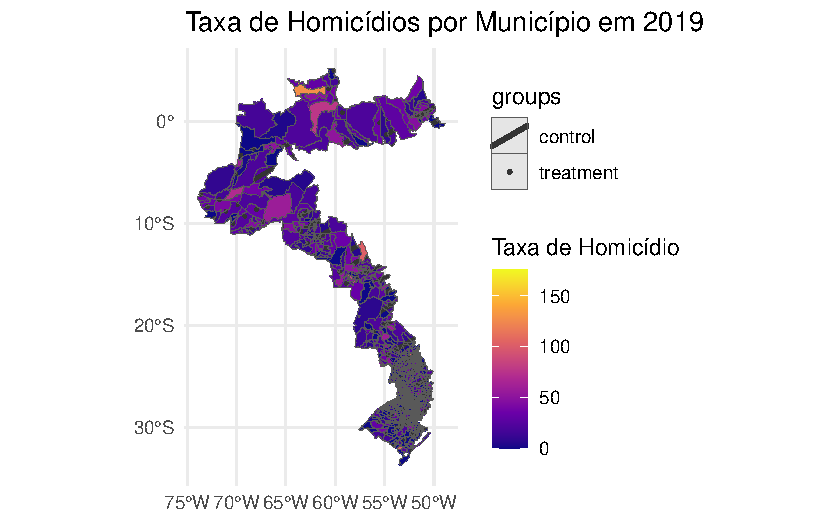
\includegraphics{maps_files/figure-pdf/unnamed-chunk-25-1.pdf}

}

\end{figure}



\end{document}
